\documentclass[journal]{IEEEtran}
\usepackage[T1]{fontenc}
\usepackage{amsmath,amsthm}
\usepackage{newtxtext,newtxmath}
\usepackage{graphicx}
\usepackage{booktabs}
\usepackage{array}
\usepackage{xcolor}
\usepackage[hidelinks]{hyperref}
\usepackage{cite}

\newtheorem{theorem}{Theorem}
\newtheorem{proposition}{Proposition}
\newtheorem{lemma}{Lemma}
\theoremstyle{definition}
\newtheorem{definition}{Definition}

\newcommand{\qAexact}{0.8183}
\newcommand{\qKexact}{0.4427}
\newcommand{\qEoneHundredK}{0.8192}
\newcommand{\qEoneTenK}{0.8064}
\newcommand{\qLSSHundredK}{0.443}
\newcommand{\chshSim}{0.8544}
\newcommand{\sideCls}{0.751}
\newcommand{\sideQ}{1.000}
\newcommand{\lyap}{0.898}
\newcommand{\lzPi}{0.892}
\newcommand{\lzLearned}{0.867}
\newcommand{\chaosAensFour}{0.999}
\newcommand{\chaosEoneFour}{0.555}
\newcommand{\chaosCHFour}{0.695}
\newcommand{\chValidN}{28}
\newcommand{\chTotalN}{44}
\newcommand{\chValidPct}{64}
\newcommand{\gapOneSmall}{0.074}
\newcommand{\gapOneBig}{0.003}
\newcommand{\gapFourSmall}{0.470}
\newcommand{\gapFourBig}{0.238}
\newcommand{\physFour}{0.996}
\newcommand{\lawGamma}{2.21}
\newcommand{\lawRatio}{2.44}
\newcommand{\lawRsq}{0.995}
\newcommand{\simConfN}{42}
\newcommand{\simConfWins}{42}
\newcommand{\simConfMeas}{+0.120}
\newcommand{\simConfTrue}{-0.017}
\newcommand{\simExMeas}{+0.190}
\newcommand{\simExTrue}{-0.114}
\newcommand{\simExFlip}{100}
\newcommand{\simIndMeas}{+0.0261}
\newcommand{\simIndTrue}{+0.0288}
\newcommand{\simCover}{0.992}
\newcommand{\eFreqAcc}{66.0}
\newcommand{\eFreqLSS}{0.000}
\newcommand{\eEBAcc}{66.2}
\newcommand{\eEBLSS}{0.045}
\newcommand{\eComboAcc}{66.8}
\newcommand{\eComboLSS}{0.063}
\newcommand{\eCtrlAcc}{67.1}
\newcommand{\eCtrlLSS}{0.056}
\newcommand{\eComboSacc}{2.3}
\newcommand{\eBeforeEdge}{+2.88}
\newcommand{\eAfterEdge}{-0.65}
\newcommand{\eEdgeRemoved}{+2.48}
\newcommand{\eEdgeKept}{+0.39}
\newcommand{\eRemovedShare}{86}
\newcommand{\eAuditK}{39}
\newcommand{\eAuditE}{2}
\newcommand{\eAuditPD}{0.105}
\newcommand{\eAuditRhoU}{0.153}
\newcommand{\eAuditLB}{-4.08}
\newcommand{\eAuditMeas}{-0.87}
\newcommand{\eAOne}{0.726}
\newcommand{\eHind}{0.790}
\newcommand{\eTie}{16.5}
\newcommand{\eTieBound}{0.917}
\newcommand{\ePowerN}{8,235}
\newcommand{\eSigCont}{26}
\newcommand{\eSigQuart}{22}
\newcommand{\eSigKept}{59}
\newcommand{\preRho}{0.89}
\newcommand{\preHits}{4}
\newcommand{\preN}{7}
\newcommand{\qMinHolm}{0.581}
\newcommand{\qNDomains}{8}
\newcommand{\ibmAmin}{0.749}
\newcommand{\ibmAmax}{0.811}
\newcommand{\ibmChshMin}{0.698}
\newcommand{\ibmChshMax}{0.836}
\newcommand{\ibmChshAbove}{7}
\newcommand{\ibmN}{8}
\newcommand{\wxN}{462,762}
\newcommand{\wxEnt}{61}
\newcommand{\wxBase}{0.262}
\newcommand{\wxAccZero}{0.742}
\newcommand{\wxAcc}{0.756}
\newcommand{\wxLSS}{0.044}
\newcommand{\wxLSSlo}{0.033}
\newcommand{\wxLSShi}{0.053}
\newcommand{\wxSacc}{0.054}
\newcommand{\wxNestLSS}{0.057}
\newcommand{\wxNestAcc}{0.758}
\newcommand{\wxGbmLSS}{0.062}
\newcommand{\wxGbmAcc}{0.760}
\newcommand{\wxEBLSS}{-0.029}
\newcommand{\wxEBAcc}{0.739}
\newcommand{\wxAOne}{0.740}
\newcommand{\wxACH}{0.795}
\newcommand{\wxKU}{0.51}
\newcommand{\wxTau}{0.96}
\newcommand{\wxLZ}{0.779}
\newcommand{\nwpN}{29,349}
\newcommand{\nwpEnt}{61}
\newcommand{\nwpBase}{0.277}
\newcommand{\nwpAccZero}{0.731}
\newcommand{\nwpAcc}{0.763}
\newcommand{\nwpLSS}{0.094}
\newcommand{\nwpLSSlo}{0.078}
\newcommand{\nwpLSShi}{0.109}
\newcommand{\nwpSacc}{0.118}
\newcommand{\nwpNestLSS}{0.098}
\newcommand{\nwpNestAcc}{0.763}
\newcommand{\nwpGbmLSS}{0.103}
\newcommand{\nwpGbmAcc}{0.758}
\newcommand{\nwpEBLSS}{0.008}
\newcommand{\nwpEBAcc}{0.741}
\newcommand{\nwpNestBLSS}{0.346}
\newcommand{\nwpNestBAcc}{0.847}
\newcommand{\nwpBenchLSS}{0.297}
\newcommand{\nwpBenchAcc}{0.840}
\newcommand{\nwpMbLSS}{0.345}
\newcommand{\nwpMbAcc}{0.847}
\newcommand{\nwpAOne}{0.734}
\newcommand{\nwpACH}{0.797}
\newcommand{\nwpKU}{0.52}
\newcommand{\nwpTau}{0.99}
\newcommand{\nwpLZ}{0.818}
\newcommand{\fbN}{29,923}
\newcommand{\fbEnt}{194}
\newcommand{\fbBase}{0.450}
\newcommand{\fbAccZero}{0.550}
\newcommand{\fbAcc}{0.643}
\newcommand{\fbLSS}{0.090}
\newcommand{\fbLSSlo}{0.078}
\newcommand{\fbLSShi}{0.103}
\newcommand{\fbSacc}{0.206}
\newcommand{\fbNestLSS}{0.090}
\newcommand{\fbNestAcc}{0.643}
\newcommand{\fbGbmLSS}{0.086}
\newcommand{\fbGbmAcc}{0.643}
\newcommand{\fbEBLSS}{0.041}
\newcommand{\fbEBAcc}{0.617}
\newcommand{\fbNestBLSS}{0.115}
\newcommand{\fbNestBAcc}{0.661}
\newcommand{\fbBenchLSS}{0.115}
\newcommand{\fbBenchAcc}{0.662}
\newcommand{\fbMbLSS}{0.115}
\newcommand{\fbMbAcc}{0.660}
\newcommand{\fbAOne}{0.609}
\newcommand{\fbACH}{0.676}
\newcommand{\fbKU}{0.35}
\newcommand{\fbTau}{0.99}
\newcommand{\hsN}{6,298}
\newcommand{\hsEnt}{479}
\newcommand{\hsBase}{0.905}
\newcommand{\hsAccZero}{0.905}
\newcommand{\hsAcc}{0.903}
\newcommand{\hsLSS}{0.172}
\newcommand{\hsLSSlo}{0.144}
\newcommand{\hsLSShi}{0.196}
\newcommand{\hsSacc}{-0.025}
\newcommand{\hsNestLSS}{0.167}
\newcommand{\hsNestAcc}{0.903}
\newcommand{\hsGbmLSS}{0.106}
\newcommand{\hsGbmAcc}{0.903}
\newcommand{\hsEBLSS}{0.003}
\newcommand{\hsEBAcc}{0.905}
\newcommand{\hsAOne}{0.905}
\newcommand{\hsACH}{0.918}
\newcommand{\hsKU}{0.64}
\newcommand{\hsTau}{0.59}
\newcommand{\prN}{459}
\newcommand{\prEnt}{51}
\newcommand{\prBase}{0.499}
\newcommand{\prAccZero}{0.501}
\newcommand{\prAcc}{0.789}
\newcommand{\prLSS}{0.314}
\newcommand{\prLSSlo}{0.226}
\newcommand{\prLSShi}{0.418}
\newcommand{\prSacc}{0.576}
\newcommand{\prNestLSS}{0.345}
\newcommand{\prNestAcc}{0.789}
\newcommand{\prGbmLSS}{0.102}
\newcommand{\prGbmAcc}{0.782}
\newcommand{\prEBLSS}{0.287}
\newcommand{\prEBAcc}{0.752}
\newcommand{\prAOne}{0.853}
\newcommand{\prACH}{0.859}
\newcommand{\prKU}{0.72}
\newcommand{\prTau}{0.98}
\newcommand{\stN}{483,488}
\newcommand{\stEnt}{110}
\newcommand{\stBase}{0.520}
\newcommand{\stAccZero}{0.518}
\newcommand{\stAcc}{0.522}
\newcommand{\stLSS}{0.000}
\newcommand{\stLSSlo}{0.000}
\newcommand{\stLSShi}{0.001}
\newcommand{\stSacc}{0.008}
\newcommand{\stNestLSS}{0.000}
\newcommand{\stNestAcc}{0.520}
\newcommand{\stGbmLSS}{-0.006}
\newcommand{\stGbmAcc}{0.516}
\newcommand{\stEBLSS}{-0.000}
\newcommand{\stEBAcc}{0.518}
\newcommand{\stAOne}{0.530}
\newcommand{\stACH}{0.526}
\newcommand{\stKU}{0.05}
\newcommand{\stTau}{0.87}
\newcommand{\stLZ}{0.500}
\newcommand{\eqN}{312,900}
\newcommand{\eqEnt}{300}
\newcommand{\eqBase}{0.312}
\newcommand{\eqAccZero}{0.722}
\newcommand{\eqAcc}{0.744}
\newcommand{\eqLSS}{0.049}
\newcommand{\eqLSSlo}{0.043}
\newcommand{\eqLSShi}{0.054}
\newcommand{\eqSacc}{0.077}
\newcommand{\eqNestLSS}{0.049}
\newcommand{\eqNestAcc}{0.744}
\newcommand{\eqGbmLSS}{0.053}
\newcommand{\eqGbmAcc}{0.745}
\newcommand{\eqEBLSS}{-0.000}
\newcommand{\eqEBAcc}{0.722}
\newcommand{\eqAOne}{0.726}
\newcommand{\eqACH}{0.773}
\newcommand{\eqKU}{0.49}
\newcommand{\eqTau}{1.01}
\newcommand{\eqActiveModLSS}{0.062}
\newcommand{\eqActiveEBLSS}{-0.000}
\newcommand{\eqQuietModLSS}{0.006}
\newcommand{\eqQuietEBLSS}{-0.000}
\newcommand{\lawA}{5.60}
\newcommand{\lawGammaTen}{2.05}
\newcommand{\lawRsqTen}{0.994}
\newcommand{\lawNstarHalf}{633}
\newcommand{\lawNstarFour}{2.1}
\newcommand{\lawBeta}{0.46}
\newcommand{\lawBetaMin}{0.33}
\newcommand{\lawGFive}{2.21}
\newcommand{\lawGloFive}{2.06}
\newcommand{\lawGhiFive}{2.36}
\newcommand{\lawGTen}{2.05}
\newcommand{\lawGloTen}{1.89}
\newcommand{\lawGhiTen}{2.21}
\newcommand{\lamD}{1.85}
\newcommand{\lamOverBeta}{1.96}
\newcommand{\lawMissPct}{19}
\newcommand{\lawMissPctB}{13}
\newcommand{\ibmQmin}{0.593}
\newcommand{\ibmQmax}{0.815}
\newcommand{\ibmQn}{32}
\newcommand{\ibmPredMAE}{0.000}
\newcommand{\eShareLo}{-498}
\newcommand{\eShareHi}{786}
\newcommand{\eRemLo}{+0.70}
\newcommand{\eRemHi}{+4.70}
\newcommand{\qSE}{0.0012}
\newcommand{\chshSE}{0.0008}
\newcommand{\chFailMinH}{0.5}
\newcommand{\chFailN}{16}
\newcommand{\chFailHgeOne}{14}
\newcommand{\wxEdgeWF}{+1.04}
\newcommand{\fbEdgeWF}{+9.03}
\newcommand{\hsEdgeWF}{-0.35}
\newcommand{\prEdgeWF}{+30.28}
\newcommand{\stEdgeWF}{+0.26}
\newcommand{\eqEdgeWF}{+1.74}
\newcommand{\eTau}{1.14}
\newcommand{\eAuditN}{82}
\newcommand{\nwpBestObs}{0.103}
\newcommand{\nwpRatio}{2.9}

\newcommand{\LorLam}{0.9046}
\newcommand{\LorDtwo}{2.06}
\newcommand{\LorBeta}{0.47}
\newcommand{\LorInvBeta}{2.14}
\newcommand{\LorG}{2.33}
\newcommand{\LorGlo}{2.06}
\newcommand{\LorGhi}{2.60}
\newcommand{\LorRsq}{0.993}
\newcommand{\LorRatio}{1.1}
\newcommand{\RosLam}{0.0706}
\newcommand{\RosDtwo}{1.83}
\newcommand{\RosBeta}{0.46}
\newcommand{\RosInvBeta}{2.18}
\newcommand{\RosG}{1.70}
\newcommand{\RosGlo}{0.86}
\newcommand{\RosGhi}{2.55}
\newcommand{\RosRsq}{0.974}
\newcommand{\RosRatio}{0.9}
\newcommand{\LfiveLam}{0.4773}
\newcommand{\LfiveDtwo}{2.42}
\newcommand{\LfiveBeta}{0.24}
\newcommand{\LfiveInvBeta}{4.17}
\newcommand{\LfiveG}{4.99}
\newcommand{\LfiveGlo}{4.72}
\newcommand{\LfiveGhi}{5.26}
\newcommand{\LfiveRsq}{0.999}
\newcommand{\LfiveRatio}{2.1}
\newcommand{\LsixLam}{0.9541}
\newcommand{\LsixDtwo}{3.68}
\newcommand{\LsixBeta}{0.18}
\newcommand{\LsixInvBeta}{5.66}
\newcommand{\LsixG}{6.79}
\newcommand{\LsixGlo}{5.34}
\newcommand{\LsixGhi}{8.23}
\newcommand{\LsixRsq}{0.995}
\newcommand{\LsixRatio}{1.8}
\newcommand{\LeightLam}{1.5915}
\newcommand{\LeightDtwo}{4.83}
\newcommand{\LeightBeta}{0.14}
\newcommand{\LeightInvBeta}{7.39}
\newcommand{\LeightG}{15.90}
\newcommand{\LeightGlo}{12.06}
\newcommand{\LeightGhi}{19.75}
\newcommand{\LeightRsq}{0.945}
\newcommand{\LeightRatio}{3.3}
\newcommand{\scaleRsqMin}{0.945}
\newcommand{\scaleRsqMax}{0.999}
\newcommand{\drRoOne}{0.305}
\newcommand{\drRoOnelo}{0.251}
\newcommand{\drRoOnehi}{0.360}
\newcommand{\drRoOneQlo}{0.263}
\newcommand{\drRoOneQhi}{0.349}
\newcommand{\drRoOneMlo}{0.231}
\newcommand{\drRoOneMhi}{0.369}
\newcommand{\drRoOneRidge}{0.310}
\newcommand{\drRoFt}{0.148}
\newcommand{\drRoFtlo}{0.104}
\newcommand{\drRoFthi}{0.200}
\newcommand{\drRoFtQlo}{0.113}
\newcommand{\drRoFtQhi}{0.186}
\newcommand{\drRoFtMlo}{0.087}
\newcommand{\drRoFtMhi}{0.211}
\newcommand{\drRoFtRidge}{0.138}
\newcommand{\drRoPers}{-0.157}
\newcommand{\drRoVsPers}{0.399}
\newcommand{\drCzOne}{0.322}
\newcommand{\drCzOnelo}{0.262}
\newcommand{\drCzOnehi}{0.382}
\newcommand{\drCzOneQlo}{0.270}
\newcommand{\drCzOneQhi}{0.368}
\newcommand{\drCzOneMlo}{0.250}
\newcommand{\drCzOneMhi}{0.387}
\newcommand{\drCzOneRidge}{0.305}
\newcommand{\drCzFt}{0.159}
\newcommand{\drCzFtlo}{0.093}
\newcommand{\drCzFthi}{0.219}
\newcommand{\drCzFtQlo}{0.109}
\newcommand{\drCzFtQhi}{0.201}
\newcommand{\drCzFtMlo}{0.075}
\newcommand{\drCzFtMhi}{0.238}
\newcommand{\drCzFtRidge}{0.150}
\newcommand{\drCzPers}{-0.024}
\newcommand{\drCzVsPers}{0.338}
\newcommand{\drSxOne}{0.096}
\newcommand{\drSxOnelo}{0.050}
\newcommand{\drSxOnehi}{0.145}
\newcommand{\drSxOneQlo}{0.056}
\newcommand{\drSxOneQhi}{0.139}
\newcommand{\drSxOneMlo}{0.050}
\newcommand{\drSxOneMhi}{0.149}
\newcommand{\drSxOneRidge}{0.087}
\newcommand{\drSxFt}{0.015}
\newcommand{\drSxFtlo}{-0.026}
\newcommand{\drSxFthi}{0.052}
\newcommand{\drSxFtQlo}{-0.014}
\newcommand{\drSxFtQhi}{0.044}
\newcommand{\drSxFtMlo}{-0.035}
\newcommand{\drSxFtMhi}{0.061}
\newcommand{\drSxFtRidge}{0.024}
\newcommand{\drSxPers}{-0.497}
\newcommand{\drSxVsPers}{0.396}
\newcommand{\drToneOne}{0.010}
\newcommand{\drToneOnelo}{-0.031}
\newcommand{\drToneOnehi}{0.054}
\newcommand{\drToneOneQlo}{-0.015}
\newcommand{\drToneOneQhi}{0.042}
\newcommand{\drToneOneMlo}{-0.055}
\newcommand{\drToneOneMhi}{0.064}
\newcommand{\drToneOneRidge}{-0.023}
\newcommand{\drToneFt}{-0.075}
\newcommand{\drToneFtlo}{-0.163}
\newcommand{\drToneFthi}{-0.011}
\newcommand{\drToneFtQlo}{-0.096}
\newcommand{\drToneFtQhi}{-0.047}
\newcommand{\drToneFtMlo}{-0.225}
\newcommand{\drToneFtMhi}{0.010}
\newcommand{\drToneFtRidge}{-0.500}
\newcommand{\drTonePers}{-0.654}
\newcommand{\drToneVsPers}{0.402}
\newcommand{\drTtwoOne}{0.044}
\newcommand{\drTtwoOnelo}{0.009}
\newcommand{\drTtwoOnehi}{0.078}
\newcommand{\drTtwoOneQlo}{0.027}
\newcommand{\drTtwoOneQhi}{0.061}
\newcommand{\drTtwoOneMlo}{-0.012}
\newcommand{\drTtwoOneMhi}{0.090}
\newcommand{\drTtwoOneRidge}{-0.030}
\newcommand{\drTtwoFt}{-0.010}
\newcommand{\drTtwoFtlo}{-0.051}
\newcommand{\drTtwoFthi}{0.022}
\newcommand{\drTtwoFtQlo}{-0.025}
\newcommand{\drTtwoFtQhi}{0.004}
\newcommand{\drTtwoFtMlo}{-0.073}
\newcommand{\drTtwoFtMhi}{0.040}
\newcommand{\drTtwoFtRidge}{-0.091}
\newcommand{\drTtwoPers}{-0.655}
\newcommand{\drTtwoVsPers}{0.423}
\newcommand{\drQubits}{467}
\newcommand{\drDays}{280}
\newcommand{\drObs}{596,938}
\newcommand{\drEdges}{1,044}
\newcommand{\drTOneObs}{69,749}
\newcommand{\drRoSecOne}{0.258}
\newcommand{\drToneSecOne}{0.089}
\newcommand{\drSecDays}{181}
\newcommand{\dbPBase}{0.178}
\newcommand{\dbPRows}{60,696}
\newcommand{\dbPBadBad}{0.539}
\newcommand{\dbPBadGood}{0.097}
\newcommand{\dbPBadBadFt}{0.495}
\newcommand{\dbPHistLSS}{0.275}
\newcommand{\dbPHistLSSlo}{0.233}
\newcommand{\dbPHistLSShi}{0.313}
\newcommand{\dbPLogitLSS}{0.310}
\newcommand{\dbPLogitLSSlo}{0.263}
\newcommand{\dbPLogitLSShi}{0.356}
\newcommand{\dbPHgbLSS}{0.324}
\newcommand{\dbPHgbLSSlo}{0.274}
\newcommand{\dbPHgbLSShi}{0.370}
\newcommand{\dbPHgbLSSMlo}{0.271}
\newcommand{\dbPHgbLSSMhi}{0.375}
\newcommand{\dbPHgbAcc}{0.887}
\newcommand{\dbPAccZero}{0.822}
\newcommand{\dbPKappa}{0.396}
\newcommand{\dbSBase}{0.194}
\newcommand{\dbSRows}{61,944}
\newcommand{\dbSBadBad}{0.578}
\newcommand{\dbSBadGood}{0.099}
\newcommand{\dbSBadBadFt}{0.534}
\newcommand{\dbSHistLSS}{0.290}
\newcommand{\dbSHistLSSlo}{0.251}
\newcommand{\dbSHistLSShi}{0.328}
\newcommand{\dbSLogitLSS}{0.352}
\newcommand{\dbSLogitLSSlo}{0.307}
\newcommand{\dbSLogitLSShi}{0.399}
\newcommand{\dbSHgbLSS}{0.361}
\newcommand{\dbSHgbLSSlo}{0.307}
\newcommand{\dbSHgbLSShi}{0.412}
\newcommand{\dbSHgbLSSMlo}{0.301}
\newcommand{\dbSHgbLSSMhi}{0.422}
\newcommand{\dbSHgbAcc}{0.885}
\newcommand{\dbSAccZero}{0.806}
\newcommand{\dbSKappa}{0.397}
\newcommand{\dbPAuc}{0.831}
\newcommand{\bellN}{300}
\newcommand{\bellK}{237}
\newcommand{\bellS}{2.35}
\newcommand{\bellSerr}{0.18}
\newcommand{\bellW}{0.790}
\newcommand{\bellWlo}{0.739}
\newcommand{\bellWhi}{0.835}
\newcommand{\bellP}{0.061}
\newcommand{\bellOwn}{0.543}
\newcommand{\bellOwnlo}{0.485}
\newcommand{\bellOwnhi}{0.601}
\newcommand{\bellSide}{0.720}
\newcommand{\bellSidelo}{0.666}
\newcommand{\bellSidehi}{0.770}
\newcommand{\bellState}{0.790}
\newcommand{\liveChsh}{0.8436}
\newcommand{\liveChshSE}{0.0029}
\newcommand{\liveTrials}{16,000}
\newcommand{\liveAqA}{0.8128}
\newcommand{\liveAqB}{0.8148}
\newcommand{\liveQA}{42}
\newcommand{\liveQB}{5}
\newcommand{\liveKappa}{0.424}
\newcommand{\liveLoss}{0.0045}
\newcommand{\liveRoMin}{0.24}
\newcommand{\liveRoMax}{0.39}
\newcommand{\liveTOneMin}{155}
\newcommand{\liveTOneMax}{277}
\newcommand{\liveDate}{2026-11-07}
\newcommand{\landDays}{253}
\newcommand{\landQubits}{155}
\newcommand{\drSecStart}{31 March 2026}
\newcommand{\drSecEnd}{27 September 2026}
\newcommand{\drToneSecOnelo}{0.029}
\newcommand{\drToneSecOnehi}{0.165}
\newcommand{\drTtwoSecOne}{0.050}
\newcommand{\drTtwoSecOnelo}{0.018}
\newcommand{\drTtwoSecOnehi}{0.079}
\newcommand{\drRoSecOnelo}{0.194}
\newcommand{\drRoSecOnehi}{0.321}
\newcommand{\lawGL}{2.44}
\newcommand{\lawGLlo}{2.27}
\newcommand{\lawGLhi}{2.61}
\newcommand{\lamCtl}{0.898}
\newcommand{\liveAboveModels}{8}
\newcommand{\liveGapTs}{0.010}
\newcommand{\liveGapTsSE}{3.5}
\newcommand{\bellWlit}{0.710}
\newcommand{\bellWlitlo}{0.655}
\newcommand{\bellWlithi}{0.761}
\newcommand{\bellPconv}{0.029}
\newcommand{\drRoHalf}{0.48}

\newcommand{\LorFloorMax}{0.0008}
\newcommand{\LorGonenn}{2.20}
\newcommand{\LorGsdonenn}{0.09}
\newcommand{\LorNidonenn}{3}
\newcommand{\LorRexponenn}{0.999}
\newcommand{\LorRpowonenn}{0.976}
\newcommand{\LorGknn}{3.31}
\newcommand{\LorGsdknn}{0.11}
\newcommand{\LorNidknn}{3}
\newcommand{\LorRexpknn}{0.996}
\newcommand{\LorRpowknn}{0.957}
\newcommand{\LorGonennTwo}{2.47}
\newcommand{\LorGonennTen}{2.24}
\newcommand{\LorGknnTwo}{--}
\newcommand{\LorGknnTen}{3.42}
\newcommand{\LorDtwolo}{2.05}
\newcommand{\LorDtwohi}{2.07}
\newcommand{\LorLamR}{0.9046}
\newcommand{\LorLamSE}{0.0008}
\newcommand{\RosFloorMax}{0.0005}
\newcommand{\RosGonenn}{1.95}
\newcommand{\RosGsdonenn}{0.32}
\newcommand{\RosNidonenn}{3}
\newcommand{\RosRexponenn}{0.960}
\newcommand{\RosRpowonenn}{0.965}
\newcommand{\RosGknn}{3.31}
\newcommand{\RosGsdknn}{0.17}
\newcommand{\RosNidknn}{3}
\newcommand{\RosRexpknn}{0.887}
\newcommand{\RosRpowknn}{0.901}
\newcommand{\RosGonennTwo}{2.14}
\newcommand{\RosGonennTen}{--}
\newcommand{\RosGknnTwo}{4.29}
\newcommand{\RosGknnTen}{--}
\newcommand{\RosDtwolo}{1.82}
\newcommand{\RosDtwohi}{1.86}
\newcommand{\RosLamR}{0.0706}
\newcommand{\RosLamSE}{0.0006}
\newcommand{\LfiveFloorMax}{0.0056}
\newcommand{\LfiveNidonenn}{0}
\newcommand{\LfiveNidknn}{0}
\newcommand{\LfiveGonennTwo}{--}
\newcommand{\LfiveGonennTen}{4.16}
\newcommand{\LfiveGknnTwo}{--}
\newcommand{\LfiveGknnTen}{--}
\newcommand{\LfiveDtwolo}{2.42}
\newcommand{\LfiveDtwohi}{2.47}
\newcommand{\LfiveLamR}{0.4773}
\newcommand{\LfiveLamSE}{0.0037}
\newcommand{\LsixFloorMax}{0.0015}
\newcommand{\LsixNidonenn}{0}
\newcommand{\LsixNidknn}{0}
\newcommand{\LsixGonennTwo}{--}
\newcommand{\LsixGonennTen}{--}
\newcommand{\LsixGknnTwo}{--}
\newcommand{\LsixGknnTen}{--}
\newcommand{\LsixDtwolo}{3.64}
\newcommand{\LsixDtwohi}{3.68}
\newcommand{\LsixLamR}{0.9541}
\newcommand{\LsixLamSE}{0.0043}
\newcommand{\LeightFloorMax}{0.0006}
\newcommand{\LeightNidonenn}{0}
\newcommand{\LeightNidknn}{0}
\newcommand{\LeightGonennTwo}{--}
\newcommand{\LeightGonennTen}{--}
\newcommand{\LeightGknnTwo}{--}
\newcommand{\LeightGknnTen}{--}
\newcommand{\LeightDtwolo}{4.78}
\newcommand{\LeightDtwohi}{4.95}
\newcommand{\LeightLamR}{1.5915}
\newcommand{\LeightLamSE}{0.0048}
\newcommand{\floorMaxAll}{0.0056}
\newcommand{\pvAgreeMin}{0.966}
\newcommand{\pvEtaDiffMax}{0.022}
\newcommand{\pvAdiffMax}{0.0080}
\newcommand{\pvFloorDiffMax}{0.0006}
\newcommand{\pvEssMed}{6171}
\newcommand{\pvPartDiff}{0.0000}
\newcommand{\pvPartAdiff}{0.000}
\newcommand{\pvDtAgree}{0.996}
\newcommand{\auND}{82}
\newcommand{\auPDw}{0.105}
\newcommand{\auDelta}{-0.87}
\newcommand{\auKUa}{10}
\newcommand{\auRhoHa}{0.122}
\newcommand{\auRhoCPa}{0.153}
\newcommand{\auLBwHa}{-6.10}
\newcommand{\auLBcpa}{-4.08}
\newcommand{\auKUb}{12}
\newcommand{\auRhoHb}{0.146}
\newcommand{\auLBwHb}{-7.14}
\newcommand{\auLBcpb}{-4.71}
\newcommand{\pwN}{8,235}
\newcommand{\pwNde}{16,470}
\newcommand{\pwGroups}{569}
\newcommand{\pwIss}{110}
\newcommand{\ecRows}{587}
\newcommand{\ecTick}{82}
\newcommand{\ecA}{+0.46}
\newcommand{\ecAlo}{-3.63}
\newcommand{\ecAhi}{+4.70}
\newcommand{\ecB}{-0.81}
\newcommand{\ecBlo}{-3.92}
\newcommand{\ecBhi}{+2.22}
\newcommand{\ecRem}{76}
\newcommand{\ecRemEdge}{+20.1}
\newcommand{\ecDiff}{-1.27}
\newcommand{\ecDifflo}{-4.47}
\newcommand{\ecDiffhi}{+1.88}
\newcommand{\auComb}{972}
\newcommand{\auAudOld}{340}
\newcommand{\auPop}{632}
\newcommand{\auIss}{90}
\newcommand{\auW}{383}
\newcommand{\auWD}{40.2}
\newcommand{\auWmin}{0.167}
\newcommand{\auPDu}{0.130}
\newcommand{\auWtopA}{10.0}
\newcommand{\auWtopB}{12.0}
\newcommand{\auTightB}{-6.49}
\newcommand{\auTightA}{-5.84}
\newcommand{\auTightWb}{1.75}
\newcommand{\auTightTopB}{9.0}
\newcommand{\auTightNun}{42}
\newcommand{\auTightKrest}{9}
\newcommand{\auEa}{2}
\newcommand{\auNa}{39}
\newcommand{\auEb}{3}
\newcommand{\auNb}{40}
\newcommand{\roA}{0.8148}
\newcommand{\roAlo}{0.8132}
\newcommand{\roAhi}{0.8164}
\newcommand{\roAez}{0.0046}
\newcommand{\roAeo}{0.0065}
\newcommand{\roAk}{0.428}
\newcommand{\roB}{0.8127}
\newcommand{\roBlo}{0.8111}
\newcommand{\roBhi}{0.8144}
\newcommand{\roBez}{0.0043}
\newcommand{\roBeo}{0.0132}
\newcommand{\roBk}{0.421}
\newcommand{\roFormulaDiff}{2.2e-05}
\newcommand{\wxTBlo}{0.055}
\newcommand{\wxTBhi}{0.060}
\newcommand{\wxTBn}{252}
\newcommand{\wxTWlo}{0.048}
\newcommand{\wxTWhi}{0.067}
\newcommand{\nwpTBlo}{0.317}
\newcommand{\nwpTBhi}{0.373}
\newcommand{\nwpTBn}{17}
\newcommand{\nwpTWlo}{0.300}
\newcommand{\nwpTWhi}{0.389}
\newcommand{\fbTBlo}{0.108}
\newcommand{\fbTBhi}{0.121}
\newcommand{\fbTBn}{169}
\newcommand{\fbTWlo}{0.098}
\newcommand{\fbTWhi}{0.131}
\newcommand{\hsTBlo}{0.127}
\newcommand{\hsTBhi}{0.201}
\newcommand{\hsTBn}{17}
\newcommand{\hsTWlo}{0.113}
\newcommand{\hsTWhi}{0.215}
\newcommand{\prTBlo}{0.050}
\newcommand{\prTBhi}{0.603}
\newcommand{\prTBn}{9}
\newcommand{\prTWlo}{0.043}
\newcommand{\prTWhi}{0.641}
\newcommand{\stTBlo}{-0.0007}
\newcommand{\stTBhi}{0.0012}
\newcommand{\stTBn}{214}
\newcommand{\stTWlo}{-0.0007}
\newcommand{\stTWhi}{0.0013}
\newcommand{\eqTBlo}{0.045}
\newcommand{\eqTBhi}{0.053}
\newcommand{\eqTBn}{80}
\newcommand{\eqTWlo}{0.041}
\newcommand{\eqTWhi}{0.056}
\newcommand{\edTBlo}{0.032}
\newcommand{\edTBhi}{0.094}
\newcommand{\edTBn}{18}
\newcommand{\edTWlo}{0.003}
\newcommand{\edTWhi}{0.128}
\newcommand{\qrevMinHolm}{0.576}
\newcommand{\qrevN}{8}
\newcommand{\qrevNsigWorse}{5}
\newcommand{\qrevStPe}{0.0025}
\newcommand{\qrevStPt}{0.072}
\newcommand{\qrevStDll}{-0.0010}
\newcommand{\qrevStLq}{+0.0002}
\newcommand{\qrevStLc}{-0.0012}
\newcommand{\qrevStCilo}{-0.0022}
\newcommand{\qrevStCihi}{+0.0005}
\newcommand{\xcN}{40}
\newcommand{\xcEpsMatch}{38}
\newcommand{\xcEpsUnchk}{2}
\newcommand{\xcGuidClean}{33}
\newcommand{\xcGuidFlagAI}{4}
\newcommand{\xcWrongFlagged}{2}
\newcommand{\xcEscreen}{7}
\newcommand{\xcKscreen}{22}
\newcommand{\xcEall}{9}
\newcommand{\xcKall}{26}
\newcommand{\xcBscreenPlain}{-12.36}
\newcommand{\xcBscreenTight}{-9.75}
\newcommand{\xcBallPlain}{-13.93}
\newcommand{\xcBallTight}{-11.23}

\newcommand{\ibInv}{76}
\newcommand{\ibIss}{31}
\newcommand{\ibIssTot}{98}
\newcommand{\ibRecur}{9}
\newcommand{\ibRecurRows}{50}
\newcommand{\ibBeatInv}{38}
\newcommand{\ibBeatVal}{59}
\newcommand{\ibEbInv}{63}
\newcommand{\ibBaseInv}{38}
\newcommand{\ibEbVal}{61}
\newcommand{\ibBaseVal}{59}
\newcommand{\ibEdgeAll}{+2.88}
\newcommand{\ibEdgeInv}{+2.48}
\newcommand{\ibEdgeVal}{+0.39}
\newcommand{\ibTfxN}{11}
\newcommand{\ibPnrN}{15}
\newcommand{\ibPnrPer}{11}
\newcommand{\ibTfxPer}{3}
\newcommand{\covIndTw}{99.8}
\newcommand{\covIndEn}{91.3}
\newcommand{\covIndTi}{90.7}
\newcommand{\covArTw}{98.6}
\newcommand{\covArEn}{88.9}
\newcommand{\covArTi}{87.6}
\newcommand{\covUwTw}{99.5}
\newcommand{\covUwEn}{89.9}
\newcommand{\covUwTi}{91.8}
\newcommand{\covMisTw}{100.0}
\newcommand{\covMisEn}{92.4}
\newcommand{\covMisTi}{92.0}
\newcommand{\covFewTw}{98.8}
\newcommand{\covFewEn}{83.9}
\newcommand{\covFewTi}{86.2}
\newcommand{\covSE}{0.4}
\newcommand{\covSEall}{1.2}
\newcommand{\covTwMin}{98.6}
\newcommand{\covOneMin}{83.9}
\newcommand{\covOneMax}{92.4}
\newcommand{\covWlo}{1.7}
\newcommand{\covWhi}{1.8}
\newcommand{\covSims}{1,000}
\newcommand{\covReps}{299}
\newcommand{\covExactMin}{95.1}
\newcommand{\AuRandP}{99.9}
\newcommand{\AuRandT}{99.9}
\newcommand{\AuHeavyP}{96.3}
\newcommand{\AuHeavyT}{96.3}
\newcommand{\AuIssP}{100.0}
\newcommand{\AuIssT}{100.0}
\newcommand{\AuUneqP}{96.2}
\newcommand{\AuUneqT}{96.2}
\newcommand{\AuUnresWP}{100.0}
\newcommand{\AuUnresWT}{100.0}
\newcommand{\AuUnresXP}{96.8}
\newcommand{\AuUnresXT}{95.8}
\newcommand{\AuMissTwentyP}{99.3}
\newcommand{\AuMissTwentyT}{99.3}
\newcommand{\AuMissFiftyP}{92.8}
\newcommand{\AuMissFiftyT}{84.9}
\newcommand{\covDrawsB}{20,000}
\newcommand{\msLoronennTwo}{2.45}
\newcommand{\msLoronennTwolo}{2.42}
\newcommand{\msLoronennTwohi}{2.49}
\newcommand{\msLoronennTwosd}{0.08}
\newcommand{\msLoronennTwon}{20}
\newcommand{\msLoronennFive}{2.22}
\newcommand{\msLoronennFivelo}{2.19}
\newcommand{\msLoronennFivehi}{2.25}
\newcommand{\msLoronennFivesd}{0.07}
\newcommand{\msLoronennFiven}{20}
\newcommand{\msLoronennTen}{2.20}
\newcommand{\msLoronennTenlo}{2.18}
\newcommand{\msLoronennTenhi}{2.23}
\newcommand{\msLoronennTensd}{0.06}
\newcommand{\msLoronennTenn}{20}
\newcommand{\msLorknnFive}{3.42}
\newcommand{\msLorknnFivelo}{3.36}
\newcommand{\msLorknnFivehi}{3.49}
\newcommand{\msLorknnFivesd}{0.16}
\newcommand{\msLorknnFiven}{20}
\newcommand{\msLorknnTen}{3.45}
\newcommand{\msLorknnTenlo}{3.42}
\newcommand{\msLorknnTenhi}{3.49}
\newcommand{\msLorknnTensd}{0.09}
\newcommand{\msLorknnTenn}{20}
\newcommand{\msLorSeeds}{20}
\newcommand{\msLorSonennTwoFull}{2.45}
\newcommand{\msLorSonennTwoFulllo}{2.42}
\newcommand{\msLorSonennTwoFullhi}{2.49}
\newcommand{\msLorSonennTwoFulln}{20}
\newcommand{\msLorSonennTwoDmin}{2.45}
\newcommand{\msLorSonennTwoDminlo}{2.42}
\newcommand{\msLorSonennTwoDminhi}{2.49}
\newcommand{\msLorSonennTwoDminn}{20}
\newcommand{\msLorSonennTwoDmax}{2.57}
\newcommand{\msLorSonennTwoDmaxlo}{2.50}
\newcommand{\msLorSonennTwoDmaxhi}{2.64}
\newcommand{\msLorSonennTwoDmaxn}{20}
\newcommand{\msLorSonennTwoLin}{2.39}
\newcommand{\msLorSonennTwoLinlo}{2.36}
\newcommand{\msLorSonennTwoLinhi}{2.43}
\newcommand{\msLorSonennTwoLinn}{20}
\newcommand{\msLorSonennFiveFull}{2.22}
\newcommand{\msLorSonennFiveFulllo}{2.19}
\newcommand{\msLorSonennFiveFullhi}{2.25}
\newcommand{\msLorSonennFiveFulln}{20}
\newcommand{\msLorSonennFiveDmin}{2.21}
\newcommand{\msLorSonennFiveDminlo}{2.19}
\newcommand{\msLorSonennFiveDminhi}{2.23}
\newcommand{\msLorSonennFiveDminn}{20}
\newcommand{\msLorSonennFiveDmax}{2.24}
\newcommand{\msLorSonennFiveDmaxlo}{2.20}
\newcommand{\msLorSonennFiveDmaxhi}{2.29}
\newcommand{\msLorSonennFiveDmaxn}{20}
\newcommand{\msLorSonennFiveLin}{2.18}
\newcommand{\msLorSonennFiveLinlo}{2.14}
\newcommand{\msLorSonennFiveLinhi}{2.22}
\newcommand{\msLorSonennFiveLinn}{20}
\newcommand{\msLorSonennTenFull}{2.20}
\newcommand{\msLorSonennTenFulllo}{2.18}
\newcommand{\msLorSonennTenFullhi}{2.23}
\newcommand{\msLorSonennTenFulln}{20}
\newcommand{\msLorSonennTenDmin}{2.19}
\newcommand{\msLorSonennTenDminlo}{2.15}
\newcommand{\msLorSonennTenDminhi}{2.23}
\newcommand{\msLorSonennTenDminn}{20}
\newcommand{\msLorSonennTenDmax}{2.20}
\newcommand{\msLorSonennTenDmaxlo}{2.18}
\newcommand{\msLorSonennTenDmaxhi}{2.23}
\newcommand{\msLorSonennTenDmaxn}{20}
\newcommand{\msLorSonennTenLin}{2.25}
\newcommand{\msLorSonennTenLinlo}{2.23}
\newcommand{\msLorSonennTenLinhi}{2.27}
\newcommand{\msLorSonennTenLinn}{20}
\newcommand{\msLorSknnTwoFulln}{0}
\newcommand{\msLorSknnTwoDminn}{0}
\newcommand{\msLorSknnTwoDmaxn}{0}
\newcommand{\msLorSknnTwoLinn}{0}
\newcommand{\msLorSknnFiveFull}{3.42}
\newcommand{\msLorSknnFiveFulllo}{3.36}
\newcommand{\msLorSknnFiveFullhi}{3.49}
\newcommand{\msLorSknnFiveFulln}{20}
\newcommand{\msLorSknnFiveDmin}{3.37}
\newcommand{\msLorSknnFiveDminlo}{3.32}
\newcommand{\msLorSknnFiveDminhi}{3.41}
\newcommand{\msLorSknnFiveDminn}{20}
\newcommand{\msLorSknnFiveDmax}{3.41}
\newcommand{\msLorSknnFiveDmaxlo}{3.29}
\newcommand{\msLorSknnFiveDmaxhi}{3.53}
\newcommand{\msLorSknnFiveDmaxn}{20}
\newcommand{\msLorSknnFiveLin}{3.44}
\newcommand{\msLorSknnFiveLinlo}{3.35}
\newcommand{\msLorSknnFiveLinhi}{3.53}
\newcommand{\msLorSknnFiveLinn}{20}
\newcommand{\msLorSknnTenFull}{3.45}
\newcommand{\msLorSknnTenFulllo}{3.42}
\newcommand{\msLorSknnTenFullhi}{3.49}
\newcommand{\msLorSknnTenFulln}{20}
\newcommand{\msLorSknnTenDmin}{3.35}
\newcommand{\msLorSknnTenDminlo}{3.32}
\newcommand{\msLorSknnTenDminhi}{3.39}
\newcommand{\msLorSknnTenDminn}{20}
\newcommand{\msLorSknnTenDmax}{3.41}
\newcommand{\msLorSknnTenDmaxlo}{3.32}
\newcommand{\msLorSknnTenDmaxhi}{3.48}
\newcommand{\msLorSknnTenDmaxn}{19}
\newcommand{\msLorSknnTenLin}{3.38}
\newcommand{\msLorSknnTenLinlo}{3.33}
\newcommand{\msLorSknnTenLinhi}{3.44}
\newcommand{\msLorSknnTenLinn}{20}
\newcommand{\msRosonennTwo}{2.18}
\newcommand{\msRosonennTwolo}{2.14}
\newcommand{\msRosonennTwohi}{2.23}
\newcommand{\msRosonennTwosd}{0.11}
\newcommand{\msRosonennTwon}{20}
\newcommand{\msRosonennFive}{1.85}
\newcommand{\msRosonennFivelo}{1.76}
\newcommand{\msRosonennFivehi}{1.95}
\newcommand{\msRosonennFivesd}{0.24}
\newcommand{\msRosonennFiven}{20}
\newcommand{\msRosknnTwo}{4.02}
\newcommand{\msRosknnTwolo}{3.86}
\newcommand{\msRosknnTwohi}{4.19}
\newcommand{\msRosknnTwosd}{0.35}
\newcommand{\msRosknnTwon}{16}
\newcommand{\msRosknnFive}{3.38}
\newcommand{\msRosknnFivelo}{3.23}
\newcommand{\msRosknnFivehi}{3.52}
\newcommand{\msRosknnFivesd}{0.35}
\newcommand{\msRosknnFiven}{20}
\newcommand{\msRosSeeds}{20}
\newcommand{\msRosSonennTwoFull}{2.18}
\newcommand{\msRosSonennTwoFulllo}{2.14}
\newcommand{\msRosSonennTwoFullhi}{2.24}
\newcommand{\msRosSonennTwoFulln}{20}
\newcommand{\msRosSonennTwoDmin}{2.23}
\newcommand{\msRosSonennTwoDminlo}{2.17}
\newcommand{\msRosSonennTwoDminhi}{2.29}
\newcommand{\msRosSonennTwoDminn}{20}
\newcommand{\msRosSonennTwoDmax}{2.18}
\newcommand{\msRosSonennTwoDmaxlo}{2.14}
\newcommand{\msRosSonennTwoDmaxhi}{2.24}
\newcommand{\msRosSonennTwoDmaxn}{20}
\newcommand{\msRosSonennTwoLin}{2.18}
\newcommand{\msRosSonennTwoLinlo}{2.14}
\newcommand{\msRosSonennTwoLinhi}{2.23}
\newcommand{\msRosSonennTwoLinn}{20}
\newcommand{\msRosSonennFiveFull}{1.85}
\newcommand{\msRosSonennFiveFulllo}{1.76}
\newcommand{\msRosSonennFiveFullhi}{1.95}
\newcommand{\msRosSonennFiveFulln}{20}
\newcommand{\msRosSonennFiveDminn}{0}
\newcommand{\msRosSonennFiveDmax}{1.85}
\newcommand{\msRosSonennFiveDmaxlo}{1.76}
\newcommand{\msRosSonennFiveDmaxhi}{1.95}
\newcommand{\msRosSonennFiveDmaxn}{20}
\newcommand{\msRosSonennFiveLin}{1.87}
\newcommand{\msRosSonennFiveLinlo}{1.77}
\newcommand{\msRosSonennFiveLinhi}{1.98}
\newcommand{\msRosSonennFiveLinn}{20}
\newcommand{\msRosSonennTenFulln}{0}
\newcommand{\msRosSonennTenDminn}{0}
\newcommand{\msRosSonennTenDmaxn}{0}
\newcommand{\msRosSonennTenLinn}{0}
\newcommand{\msRosSknnTwoFull}{4.02}
\newcommand{\msRosSknnTwoFulllo}{3.86}
\newcommand{\msRosSknnTwoFullhi}{4.19}
\newcommand{\msRosSknnTwoFulln}{16}
\newcommand{\msRosSknnTwoDmin}{4.02}
\newcommand{\msRosSknnTwoDminlo}{3.86}
\newcommand{\msRosSknnTwoDminhi}{4.19}
\newcommand{\msRosSknnTwoDminn}{16}
\newcommand{\msRosSknnTwoDmaxn}{0}
\newcommand{\msRosSknnTwoLin}{3.98}
\newcommand{\msRosSknnTwoLinlo}{3.82}
\newcommand{\msRosSknnTwoLinhi}{4.16}
\newcommand{\msRosSknnTwoLinn}{16}
\newcommand{\msRosSknnFiveFull}{3.38}
\newcommand{\msRosSknnFiveFulllo}{3.22}
\newcommand{\msRosSknnFiveFullhi}{3.52}
\newcommand{\msRosSknnFiveFulln}{20}
\newcommand{\msRosSknnFiveDmin}{2.81}
\newcommand{\msRosSknnFiveDminlo}{2.65}
\newcommand{\msRosSknnFiveDminhi}{2.97}
\newcommand{\msRosSknnFiveDminn}{19}
\newcommand{\msRosSknnFiveDmax}{3.50}
\newcommand{\msRosSknnFiveDmaxlo}{3.20}
\newcommand{\msRosSknnFiveDmaxhi}{3.79}
\newcommand{\msRosSknnFiveDmaxn}{20}
\newcommand{\msRosSknnFiveLin}{3.38}
\newcommand{\msRosSknnFiveLinlo}{3.22}
\newcommand{\msRosSknnFiveLinhi}{3.53}
\newcommand{\msRosSknnFiveLinn}{20}
\newcommand{\msRosSknnTenFulln}{0}
\newcommand{\msRosSknnTenDminn}{0}
\newcommand{\msRosSknnTenDmaxn}{0}
\newcommand{\msRosSknnTenLinn}{0}
\newcommand{\rpN}{551}
\newcommand{\rpPass}{551}
\newcommand{\rpMaxRel}{0.0e+00}
\newcommand{\rpTol}{relative 1e-9 or absolute 1e-12}

\newcommand{\kLam}{0.898}
\newcommand{\kQa}{0.8183}
\newcommand{\kLzTinyEight}{0.981}
\newcommand{\kLzOneEight}{0.490}
\newcommand{\kLzTinyFour}{0.999}
\newcommand{\kLzOneFour}{0.539}
\newcommand{\kLzOneOne}{0.843}
\newcommand{\kLTinyEight}{7.2}
\newcommand{\kLFour}{3.6}
\newcommand{\kQsigOne}{0.707}
\newcommand{\kQsigTenth}{0.818}
\newcommand{\kLZpi}{0.892}
\newcommand{\kLZlearn}{0.867}
\newcommand{\kLZbase}{0.515}
\newcommand{\kDepTwo}{0.755}




\newcommand{\E}{\mathbb{E}}
\newcommand{\F}{\mathcal{F}}
\newcommand{\LSS}{\mathrm{LSS}}
\newcommand{\KL}{\mathrm{KL}}
\newcommand{\ind}{\mathbf{1}}
\newcommand{\Hb}{H_{\mathrm b}}

\begin{document}

\title{How Much of the Future Is Knowable? Information Ceilings, Chaos, Label Errors and Quantum Resources}

\author{Johan~Abraham%
\thanks{J. Abraham is an independent researcher. Code, derived results and the audit materials are public at \url{https://github.com/6866561/knowability-illusory-edge} (Appendix~\ref{app:repro}). A companion paper~\cite{abraham2026illusory} develops the label-error results in Section~\ref{sec:res-self} in detail.}}

\markboth{Preprint, November 2026}{Abraham: How Much of the Future Is Knowable?}

\maketitle

\begin{abstract}
Whether mathematics can predict the future depends on the event, the information available and what counts as success. We treat knowability as the Bayes ceiling of a stated information set and write the expected measured loss of any forecast as three nonnegative parts (randomness irreducible under a stated physical model and information access, missing information, model error) plus a signed distortion from label errors. The identity organises these parts but does not measure them, so each is examined where other evidence pins it down. Under quantum theory a qubit's ceiling of $\qAexact$ does not improve with more precise knowledge of its preparation; a live IBM processor's measured response implies $\roA$. In Lorenz-63 an ensemble forecast $\kLTinyEight$ Lyapunov times ahead is right $\kLzOneEight$ of the time, indistinguishable from a coin, with observation noise $1$, and $\kLzTinyEight$ with noise $10^{-4}$, while the data a nearest-neighbour learner needs grow steeply with the horizon. In nine real forecasting tasks, achieved skill over point-in-time base rates ranges from $\nwpNestBLSS$ for rain with weather-model input to indistinguishable from zero for stock direction. Persistent label errors can manufacture edge that time-ordered validation misses; in an earnings model the apparent advantage sat in invalid rows, and an audit could not certify a positive edge. Quantum computation cannot raise a classical information ceiling, and simulated quantum classifiers showed no detectable advantage in eight domains; quantum resources change predictability only by changing information, through entanglement. Next-calibration readout errors of IBM processors are partly forecastable, coherence times at most weakly.
\end{abstract}

\begin{IEEEkeywords}
Predictability, Bayes error, information theory, chaos, forecast verification, label noise, quantum information, philosophy of prediction.
\end{IEEEkeywords}

\section{Introduction}
\IEEEPARstart{A}{} forecasting model that is right more often than a coin invites a large conclusion: that mathematics can, at least partly, foresee events. The conclusion does not follow. A model that predicts ``no rain'' every day in a dry city beats a coin without knowing anything about tomorrow; a model that scores well against mislabelled outcomes may have learned the mislabelling; and a model that cannot beat the base rate may still be facing an outcome that is predictable from information it was not given. Whether, and how much, the future can be known is a question about three things at once: the event, the information available about it at the time of the forecast, and the reference against which success is judged.

This paper treats that question as a measurement problem. The quantity of interest is the \emph{Bayes ceiling} of an information set, which we compute exactly or approximately in controlled systems and bound only indirectly, through achieved skill, on real tasks: the best accuracy, or the smallest expected loss, that any decision rule using that information can achieve. The ceiling is not a property of an event alone; the same election is barely predictable from last year's result and almost certain from tomorrow's ballots. Asking ``how much of the future is knowable'' therefore means asking how much a given body of information can remove, where the remainder comes from, and how far real forecasts fall short of the ceiling and why.

The question has a long history in philosophy and physics, and those traditions disagree about where the limits lie. Laplace located them in human ignorance~\cite{laplace1814essai}; Poincar\'e and Lorenz showed that ignorance grows with time in chaotic systems~\cite{poincare1908science,lorenz1963deterministic}; quantum theory, on its standard reading, places a limit in nature itself~\cite{bell1964einstein}; Hume questioned whether past regularities license any forecast~\cite{hume1748enquiry}; and studies of forecasters found that people routinely overstate what they know~\cite{kahneman1973psychology,meehl1954clinical,tetlock2015superforecasting}. We organise these perspectives around one exact identity (Proposition~\ref{prop:anat}): the expected measured log loss of any forecast is the sum of an \emph{ontic} term (randomness that no information in a stated set $\F_\infty$ removes, under a stated physical model), an \emph{epistemic} term (information that exists but is not used), a \emph{model} term (the forecast's distance from the best use of its information) and a signed \emph{measurement} distortion (errors in the recorded outcomes, which can make measured loss look better or worse). The identity organises these components; it does not identify their values without further information, which is why each is studied where it can be pinned down. Each term is then studied where it can be isolated: a qubit for the ontic term, chaotic flows for the epistemic and model terms, nine real forecasting tasks for informational limits, and a production earnings model for measurement. Quantum computing enters twice, as a test of whether more computation can raise a ceiling and as a resource that changes the information itself.

\subsection{Contributions and their status}
Each item is marked as established (E), synthesis (S), new proposition (N) or new empirical finding (F).
\begin{enumerate}
\item (S) A four-term decomposition of forecast loss that maps the classical perspectives on predictability onto measurable quantities (Section~\ref{sec:framework}); the components are standard (Theil's uncertainty coefficient~\cite{theil1970estimation}, log-loss decompositions~\cite{weijs2010kl,roulston2002evaluating}), the organisation is ours.
\item (F) A direct comparison of ontic and epistemic limits on the same scale: the qubit ceiling saturates as knowledge sharpens, the chaotic ceiling approaches one, and a live IBM processor sits just below the qubit ceiling (Section~\ref{sec:res-demon}).
\item (F, exploratory) Learnability--horizon curves for two nearest-neighbour learners in five chaotic systems, with seeds, floors and crossing classification (Section~\ref{sec:res-chaos}).
\item (F) Achieved skill relative to point-in-time base rates in nine forecasting tasks, with entity and time-block uncertainty (Section~\ref{sec:res-atlas}).
\item (N) An inflation identity and sign-reversal construction for entity-persistent label errors, conditions under which time-ordered validation cannot detect them, and a disagreement audit with a finite-population guarantee (Section~\ref{sec:res-self}; detailed in~\cite{abraham2026illusory}).
\item (E/F) The classical-input ceiling for quantum models (a data-processing corollary), a validation-selected comparison of quantum and classical classifiers in eight domains, a live CHSH experiment, a reanalysis of a loophole-free Bell test, and forecasts of IBM processor calibrations (Sections~\ref{sec:res-qc}--\ref{sec:res-drift}).
\end{enumerate}

\section{Perspectives on the Knowability of the Future}\label{sec:perspectives}
Each perspective below is reduced to a question the data can address; Table~\ref{tab:persp} lists the questions, where they are tested and what was found.

\emph{Determinism and Laplace's demon.} Laplace imagined an intellect that knew the positions and forces of all things and for which ``nothing would be uncertain''~\cite{laplace1814essai}. In the terms of Proposition~\ref{prop:anat}, determinism says the ontic term is zero and every limit is epistemic. The testable consequence is that the ceiling should approach one as knowledge of the present improves.

\emph{Sensitive dependence.} Poincar\'e noted that small differences in initial conditions can produce very large ones in outcomes~\cite{poincare1908science}, and Lorenz turned the observation into a finite predictability horizon for weather~\cite{lorenz1963deterministic,lorenz1969predictability}. Determinism survives, but the precision needed for a fixed horizon grows exponentially, at a rate set by the largest Lyapunov exponent $\lambda$. Two questions follow: how precision trades against horizon, and how much \emph{data} a learner needs to approach the ceiling as the horizon grows.

\emph{Ontic randomness.} Quantum measurement outcomes are, according to quantum theory, not determined by the preparation; Bell showed that no local hidden-variable theory reproduces the theory's correlations~\cite{bell1964einstein}, and loophole-free tests confirm the violation~\cite{hensen2015loophole,hensen2016second}. Bell violations rule out locally causal completions under the assumptions of the tests; they do not by themselves show that every completion of quantum mechanics is indeterministic~\cite{norsen2011local}. Under quantum theory with access only to the preparation, the ontic term is positive and the ceiling stays below one however precisely the preparation is known.

\emph{Induction and stationarity.} Hume argued that no amount of past regularity entails a future one~\cite{hume1748enquiry}. Statistically, every forecast assumes that the relation learned from the past persists. The question is not whether induction is justified in general but how far forecasts evaluated strictly forward in time, on data they never saw, retain the skill they show in sample.

\emph{Falsifiability.} Popper required scientific claims to state what would refute them~\cite{popper1959logic}. A claim that the future is knowable to a stated degree can be put in that form: predicted skill ranges, fixed before the data are seen, can fail. We preregistered six hypotheses with failure conditions and report the outcome of each.

\emph{Base rates and human judgement.} People neglect base rates when they predict~\cite{kahneman1973psychology}; simple statistical rules match or beat expert judgement in many fields~\cite{meehl1954clinical}; and trained forecasters can be calibrated but rarely see far ahead~\cite{tetlock2015superforecasting}. The quantitative counterpart is the gap between raw accuracy and skill over the base rate.

\emph{Reflexive systems.} In markets, a forecast that is widely acted on changes the price it forecasts. Efficient-market theory predicts little exploitable predictability from public information~\cite{fama1970efficient}, though not none, since information is costly to acquire~\cite{grossman1980impossibility}. The question is whether next-day direction is forecastable from public price history at all.

\emph{Self-deception in measurement.} A forecast's record is only as good as the outcomes it is scored on. Leakage and label errors can make an edge appear where none exists~\cite{kapoor2023leakage,northcutt2021pervasive}. Here the question is how large the measurement term can be, whether standard validation catches it, and how to bound it cheaply.

\emph{Information versus computation.} If the ceiling is set by information, more computation can only bring a forecast closer to it. Quantum computers are often presented as a route to new predictive power; data processing, with Holevo's bound for the quantum step~\cite{holevo1973bounds}, implies that on classical inputs they cannot exceed the classical Bayes ceiling. The open question is empirical: whether, below the ceiling, quantum models fit real forecasting data better.

\emph{Quantum side information.} What quantum resources can change is the information itself. A forecaster holding a system entangled with the one being measured can predict outcomes that no classical record of the past allows~\cite{berta2010uncertainty}; the CHSH game makes the gain operational~\cite{clauser1969proposed,tsirelson1980quantum}. The question is how much of that gain survives on real hardware and in a loophole-free experiment.

\begin{table*}[!t]
\caption{Perspectives on Predictability, the Questions They Pose and What Was Found}
\label{tab:persp}
\centering
\footnotesize
\renewcommand{\arraystretch}{1.12}
\begin{tabular}{@{}p{0.15\textwidth}p{0.27\textwidth}p{0.08\textwidth}p{0.43\textwidth}@{}}
\toprule
Perspective & Question & Where & Finding\\
\midrule
Laplace's demon & Does the ceiling approach one as knowledge of the present improves? & \ref{sec:res-demon} & Yes for Lorenz-63 (ensemble-rule accuracy $\kLzOneEight\to\kLzTinyEight$ at $\kLTinyEight$ Lyapunov times as noise falls from $1$ to $10^{-4}$, approximate posterior); no for the qubit under quantum theory (saturates at $\qAexact$).\\
Sensitive dependence & How fast do precision and data requirements grow with horizon? & \ref{sec:res-demon}, \ref{sec:res-chaos} & Precision buys horizon roughly logarithmically; data needs grow steeply with horizon at rates that depend on the learner ($\LorGonenn$ vs $\LorGknn$ per Lyapunov time for Lorenz-63).\\
Ontic randomness & Is there a floor that no information about the present removes? & \ref{sec:res-demon}, \ref{sec:res-side} & Under quantum theory, qubit ceiling $\qAexact$ (knowable fraction $\qKexact$); live processor $\roA$; Bell data inconsistent with locally causal completions under the test's assumptions.\\
Induction & Does skill survive strictly forward evaluation? & \ref{sec:res-atlas} & Positive forward skill in eight of nine tasks; stock skill indistinguishable from zero under time-block resampling.\\
Falsifiability & Do preregistered predictions hold? & \ref{sec:res-prereg} & Ranking held ($\rho=\preRho$); only $\preHits$ of $\preN$ point intervals contained the result; one hypothesis component failed.\\
Base rates & Is high accuracy high skill? & \ref{sec:res-atlas} & No: House seats are called correctly $\hsAcc$ of the time but the base rate already gives $\hsAccZero$.\\
Reflexive systems & Is next-day market direction forecastable from price history? & \ref{sec:res-atlas} & Skill $\stLSS$, interval including zero.\\
Self-deception & How large can measurement error make an edge? & \ref{sec:res-self} & Removed mislabelled rows carried $\ecRemEdge$ points; the audit could not certify a positive edge.\\
Computation & Do quantum models fit classical data better? & \ref{sec:res-qc} & No significant advantage in $\qrevN$ domains (smallest Holm $p=\qrevMinHolm$).\\
Side information & Does entanglement change what is predictable in practice? & \ref{sec:res-side} & CHSH win rate $\liveChsh$ on hardware and $\bellW$ in a loophole-free test (heralded convention), against $0.75$ for classical strategies.\\
\bottomrule
\end{tabular}
\end{table*}

\section{Related Work}\label{sec:related}
\emph{Limits of predictability.} Entropy-rate bounds on predictability were estimated for human mobility~\cite{song2010limits} and debated for their estimators~\cite{xu2019predictability}; limits for social outcomes were examined through large prediction challenges and simulations~\cite{salganik2020measuring,martin2016exploring,hofman2017prediction}. Weather predictability was framed by Lorenz~\cite{lorenz1969predictability}, quantified for midlatitude weather~\cite{zhang2019predictability}, and its practical progress reviewed in~\cite{bauer2015quiet}. These studies address one domain or one estimator; we compare domains, controls and quantum systems under one protocol.

\emph{Scoring and information.} Proper scoring rules~\cite{gneiting2007strictly,brier1950verification} and their information-theoretic decompositions~\cite{weijs2010kl,roulston2002evaluating} underlie the skill measures; the knowable fraction is Theil's uncertainty coefficient~\cite{theil1970estimation}. Nearest-neighbour error bounds~\cite{cover1967nearest,hellman1970probability} are used only as diagnostics.

\emph{Label errors and leakage.} Instance-dependent label noise is surveyed in~\cite{frenay2014survey,song2023learning}; errors in benchmark test sets change model rankings~\cite{northcutt2021pervasive}; leakage undermines machine-learning-based science~\cite{kapoor2023leakage}.

\emph{Quantum machine learning and quantum information.} Rigorous advantages exist for constructed problems~\cite{liu2021rigorous} and in sample complexity for some tasks~\cite{huang2021information}; careful benchmarking finds little advantage on standard data~\cite{bowles2024better}. The operational meaning of conditional min-entropy~\cite{konig2009operational}, entropic uncertainty with quantum memory~\cite{berta2010uncertainty} and the drift of superconducting qubits~\cite{klimov2018fluctuations,burnett2019decoherence,carroll2022dynamics,proctor2020detecting} provide the context for the quantum sections.

\section{A Framework for Knowability}\label{sec:framework}
Formal definitions and proofs are in Appendix~\ref{app:math}.

\emph{Information sets and ceilings.} A forecasting task specifies an evaluation distribution $P$ of a test example $(X,Y)$, where $X$ collects everything available at the decision time and $Y\in\{0,1\}$ with $0<P(Y=1)<1$. The Bayes ceiling of the information set $\F=\sigma(X)$ is
\begin{equation}
A^*(\F)=\E\max\{\eta(X),1-\eta(X)\},\quad \eta(x)=P(Y=1\mid X=x).
\end{equation}
No decision rule using only $X$, deterministic or randomised, exceeds it (Lemma~\ref{lem:app1}). The ceiling belongs to the information set and the distribution, not to the event: enlarging $\F$ can only raise it.

\emph{Knowable fraction.} The information-theoretic counterpart is $\kappa(\F)=I(Y;X)/H(Y)\in[0,1]$, the share of the outcome's entropy that the information removes~\cite{theil1970estimation}. It equals one for a determined outcome and zero for one independent of the information.

\emph{Learnability.} A ceiling says what is possible with unlimited data. For a named learning algorithm $\mathcal A$ trained on $n$ examples, $A_n(\mathcal A)=\E_{S_n}\Pr\{\mathcal A(S_n)(X)=Y\}$ and the gap is $G_n(\mathcal A)=A^*(\F)-A_n(\mathcal A)$. Finite-sample statements concern specific algorithms; we make no claim about an optimal learner.

\emph{Anatomy of unpredictability.} Let $\F_\infty\supseteq\F$ be a larger information set, generated by $X$ together with further variables $Z$; in principle $\F_\infty$ can contain everything about the present state of the world that physics allows to be known.

\begin{proposition}[Four-term decomposition]\label{prop:anat}
For a forecast $\hat p$ that uses only $X$ (given its training data), scored against recorded labels $\tilde Y$, the expected measured log loss is
\begin{multline}\label{eq:anat}
\E\,\ell(\hat p,\tilde Y)=\underbrace{H(Y\mid\F_\infty)}_{\text{ontic}}+\underbrace{I(Y;Z\mid X)}_{\text{epistemic}}\\
+\underbrace{\E\,\KL(\eta\Vert\hat p)}_{\text{model}}+\underbrace{M}_{\text{measurement}},
\end{multline}
where $M=\E\big[(\tilde Y-Y)\ln\{(1-\hat p(X))/\hat p(X)\}\big]$. The first three terms are nonnegative; $M$ is signed.
\end{proposition}
The proof is short (Proposition~\ref{prop:appanat}). Label errors can make measured loss look better ($M<0$, when recorded labels agree with the forecast more than true ones) or worse ($M>0$), so $M$ is a distortion, not a loss. The identity is an accounting of components; on real tasks none of the terms is observed separately without further information (a known ceiling, an exact reference, or audited labels). Each term answers to a perspective of Section~\ref{sec:perspectives}. Determinism asserts that the ontic term vanishes when $\F_\infty$ is the exact present state; quantum theory, with $\F_\infty$ containing the preparation, asserts that it does not. Sensitive dependence makes the epistemic term grow with the horizon for fixed measurement precision. The model term is what learning theory studies and what more data or computation can reduce; quantum models act only here. The measurement term is what self-deception exploits. Which part of a loss counts as ontic depends on what $\F_\infty$ contains and on the physical model; we use ``ontic'' to mean irreducible under the stated quantum model and information access, not a claim that every completion of quantum mechanics is indeterministic~\cite{norsen2011local}.

\emph{Achieved skill.} Real forecasts are compared with a point-in-time base-rate forecast $p_0$ through the empirical log-loss skill $\widehat{\LSS}=1-\overline{\ell}(\hat p)/\overline{\ell}(p_0)$, a ratio of test-set averages that, for i.i.d.\ test examples from a fixed distribution (or under stationarity and ergodicity), converges to the population ratio of expected losses,
\begin{equation}\label{eq:lss}
\LSS=1-\frac{H(Y\mid X)+\E\,\KL(\eta\Vert\hat p)}{H(Y\mid\F_0)+\E\,\KL(\eta_0\Vert p_0)},
\end{equation}
although under drift or strong dependence it need not converge, and its finite-sample expectation generally differs from that ratio. Achieved skill thus mixes the information gained over the base rate with the model terms of both forecasts. A small LSS is not evidence of a small ceiling, and an achieved score improvement from adding a block of inputs is not a conditional mutual information; it can be negative.

\emph{Closed forms.} For a qubit prepared as $R_y(\theta)\lvert0\rangle$ with $\theta\sim U(0,\pi)$ known exactly, $A^*=\tfrac12+\tfrac1\pi$ and $\kappa=1/\ln2-1$; with readout errors the ceiling has the closed form of Proposition~\ref{prop:appqubit}. For exchangeable entities with Beta-distributed rates, the finite-history Bayes accuracy has the closed form of Proposition~\ref{prop:appbeta}. On a classical input, conditionally on the training data, any quantum model is a randomised function of that input and cannot exceed its Bayes ceiling (Proposition~\ref{prop:appqc}).

\section{Experimental Design}\label{sec:design}
\emph{Controls.} The ontic control is the qubit above, with the preparation angle observed exactly or with Gaussian noise $\sigma_\theta$. The epistemic controls are chaotic flows: Lorenz-63 with observation noise $\sigma_o\in\{10^{-4},\ldots,1\}$ and horizons up to eight time units, with a 400-particle ensemble reference, and, for learnability, Lorenz-63, R\"ossler and Lorenz-96 with five, six and eight variables (Section~\ref{sec:res-chaos}).

\emph{Real tasks.} Measurable rain at 61 stations (with a numerical-weather-prediction, NWP, benchmark over 17 months), football home wins (with closing odds), contested U.S.\ House seats and presidential state outcomes, earnings guidance, next-day direction of large U.S.\ stocks and funds, weekly earthquake occurrence in $2^\circ$ cells, and out-of-tolerance events in IBM processor calibrations.

\emph{Protocol.} Every real task is evaluated walk-forward and point in time: a row is scored only by models fitted on labels available before its decision time, and all preprocessing is fitted on training data only. Models are the point-in-time base rate, an empirical-Bayes entity model~\cite{robbins1956empirical,efron1975data}, $L_2$ logistic regression, gradient boosting and nested variants that take the base-rate forecast as input. A feature-and-timestamp specification with a leakage audit is part of the reproducibility package; no leakage was demonstrated, and unresolved risks are listed in Section~\ref{sec:threats}.

\emph{Inference.} Achieved-skill intervals resample entities, contiguous time blocks (calendar month, election year or quarter), and both together; the two-way (pigeonhole) bootstrap~\cite{owen2007pigeonhole} is primary because forecast errors share both entity and calendar shocks. A coverage study of the LSS ratio itself (Appendix~\ref{app:coverage}; $\covSims$ simulated panels per scenario) found two-way coverage of at least $\covTwMin\%$ at nominal $95\%$ under independent and autocorrelated calendar shocks, unequal weights, missing cells and eight time clusters, against $\covOneMin$--$\covOneMax\%$ for one-way resampling; the two-way intervals are conservative, $\covWlo$--$\covWhi$ times as wide. Quantum and classical models are selected within each family on a held-out validation split and tested once; comparisons use entity and month-block bootstraps, a one-sided Diebold--Mariano test~\cite{diebold1995comparing}, and Holm's correction~\cite{holm1979simple} over the eight domains applied to the larger of the two bootstrap $p$-values.

\emph{Preregistration.} Hypotheses H1--H6 with failure conditions, primary models and predicted skill ranges were fixed in a document whose SHA-256 hash was committed to a local repository before the new real-task data were downloaded. The hash identifies the content; the commit time is not independently verifiable. Analyses added later are labelled exploratory.

\section{Results}\label{sec:results}

\subsection{Ontic and epistemic limits: the demon's test}\label{sec:res-demon}
Fig.~\ref{fig:demon} puts the two kinds of limit on one scale. In Lorenz-63, a deterministic system, the accuracy of the ensemble forecast at a fixed horizon rises towards one as observation noise falls: at $\kLTinyEight$ Lyapunov times it is $\kLzOneEight$ ($\kLzOneEightlo$--$\kLzOneEighthi$ over $\kNtest$ test states) with $\sigma_o=1$, indistinguishable from a coin, and $\kLzTinyEight$ ($\kLzTinyEightlo$--$\kLzTinyEighthi$) with $\sigma_o=10^{-4}$; at $\kLFour$ Lyapunov times it rises from $\kLzOneFour$ to $\kLzTinyFour$. Each tenfold gain in precision extends the horizon at which a given accuracy holds by a roughly constant amount (Fig.~\ref{fig:demon}a), as expected when errors grow like $e^{\lambda t}$ with $\lambda=\kLam$. These are finite-sample accuracies of a 400-particle ensemble rule built on the local flat-prior approximation of Section~\ref{sec:res-chaos}, not population Bayes ceilings (which cannot fall below $0.5$), and the approximation has not been validated directly in this tiny-noise, long-horizon regime. With those qualifications, Laplace's claim holds here in the form chaos allows: perfect knowledge would give perfect prediction, and every finite precision gives a finite horizon.

The qubit behaves differently. With the preparation angle known to within $\sigma_\theta=0.1$ radians the ceiling is $\kQsigTenth$, and with exact knowledge it is $\qAexact$; it never approaches one (Fig.~\ref{fig:demon}b). The remaining share $1-\kappa$ of the outcome's entropy, with $\kappa=\qKexact$, is not removed by any knowledge of the preparation under quantum theory; with $\F_\infty$ containing the preparation, this is the ontic term of Proposition~\ref{prop:anat}. On IBM's ibm\_kingston processor, the measured response of two qubits implies ceilings of $\roB$ ($\roBlo$--$\roBhi$) and $\roA$ ($\roAlo$--$\roAhi$), slightly below the ideal because of readout errors ($e_0=\roBez$, $e_1=\roBeo$ and $e_0=\roAez$, $e_1=\roAeo$). Depolarizing noise lowers the ceiling further ($\kDepTwo$ at strength $0.2$). The fitted readout channels and the depolarizing noise considered here lower the average ceiling relative to the ideal preparation ensemble. This is not true of every channel: a reset channel that always returns $\lvert0\rangle$ makes the recorded outcome perfectly predictable while destroying information about the intended measurement.

On the qubit, a gradient-boosting learner reached $\qEoneHundredK$ (standard error $\qSE$) with $10^5$ examples, within sampling error of the exact accuracy ceiling. Accuracy alone does not show that probabilities are right, so we also computed the model term $\E\,\KL(\eta\Vert\hat p)$ exactly from the known $\eta(\theta)$ on $200{,}000$ held-out angles: it falls from $\kMtOneK$ nats with $10^3$ training examples to $\kMtTenK$ with $10^4$ and $\kMtHundredK$ with $10^5$ (largest upper 95\% limit over three seeds $\kMtHundredKhi$), or $\kMtShare\%$ of the exact conditional entropy $\kHcond$. Where the information is this simple, the model term can be driven close to zero in log-loss terms. Table~\ref{tab:controls} gives the reference values; the nearest-neighbour plug-in diagnostics in the table are asymptotic and fell below the ensemble reference in $\chFailN$ of 44 chaos settings, so they are not bounds.

\begin{figure*}[!t]
\centering
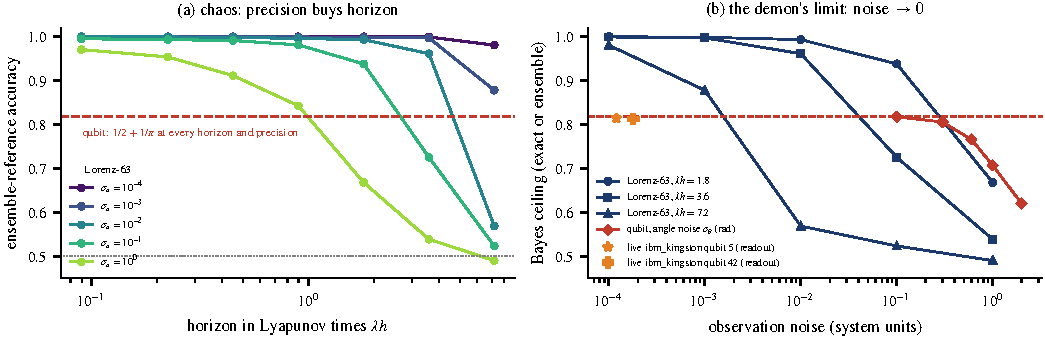
\includegraphics[width=\textwidth]{figs/fig_demon.pdf}
\caption{Ontic and epistemic limits. (a)~Lorenz-63: finite-sample accuracy ($\kNtest$ test states) of the 400-particle ensemble rule against horizon in Lyapunov times, for five levels of observation noise $\sigma_o$; dashed: the exact qubit ceiling $\tfrac12+\tfrac1\pi$, which does not depend on horizon. (b)~Against observation noise: the Lorenz-63 ensemble-rule accuracy at three horizons approaches one as noise falls; the exact qubit ceiling with angle noise $\sigma_\theta$ saturates at $\tfrac12+\tfrac1\pi$ (dashed); stars: live ibm\_kingston qubits, whose ceilings are lowered by readout error. Noise units differ between systems (state units for Lorenz-63, radians for the qubit).}
\label{fig:demon}
\end{figure*}

\begin{table}[!t]
\caption{Controls: Reference Values and Plug-in Diagnostics}
\label{tab:controls}
\centering
\scriptsize
\setlength{\tabcolsep}{2.2pt}
\begin{tabular}{@{}lcccccc@{}}
\toprule
Setting & $A^*$ ref. & $A_{\rm learn}$ & CH diag. & $\kappa$ ref. & LSS & $\kappa_U$ diag.\\
\midrule
\csname @@input\endcsname gen/tab_controls.tex
\bottomrule
\end{tabular}
\vspace{2pt}

\parbox{\columnwidth}{\scriptsize Reference: exact (qubit) or 400-particle ensemble estimate (Lorenz). CH and $\kappa_U$: asymptotic plug-in diagnostics from finite-sample 1-NN errors, not bounds.}
\end{table}

\subsection{The cost of horizon: learning chaotic futures}\label{sec:res-chaos}
A ceiling assumes the forecaster knows the dynamics. A forecaster who must learn them from data faces the model term, and in chaotic systems it grows with the horizon. For five systems we drew three independent datasets each and measured, for $n$ from $10^3$ to $10^6$, the accuracy gap between an ensemble reference and two learners, 1-NN and $k$-NN with $k=\lceil\sqrt n\rceil$, for the sign of the first coordinate $0.5$ to $3$ Lyapunov times ahead (Fig.~\ref{fig:law3}, Table~\ref{tab:law3}). Observations carry noise $10^{-4}$ times each coordinate's standard deviation. The reference is the fraction of 500 particles, drawn around the observation and integrated forward, that satisfy the target; for Lorenz-63 it agreed with an importance-sampled posterior over $2\times10^7$ invariant-measure samples in at least $\pvAgreeMin$ of decisions at larger noise, and was stable to particle number and step size at the study's noise. Particle number and step size check numerical stability within this approximation, not the posterior assumption, and the tiny-noise regime and the other systems were not validated directly, so all results are gaps to the ensemble reference. The 1-NN learner is not consistent; computed from the same approximate posterior, its asymptotic excess error $\E[r(1-2r)]$ is at most $\floorMaxAll$, far below the tolerance of $0.05$, so the crossings are attainable conditional on the reference model.

The sample size $n^*$ at which the gap reaches $0.05$ grows steeply with the horizon. For Lorenz-63 the growth is close to exponential (mean $R^2$ of an exponential fit $\LorRexponenn$ against $\LorRpowonenn$ for a power law in the horizon), at $\gamma_L=\LorGonenn\pm\LorGsdonenn$ per Lyapunov time for 1-NN and $\LorGknn\pm\LorGsdknn$ for $k$-NN (mean $\pm$ s.d.\ over three seeds, a descriptive spread rather than a full interval); for R\"ossler the rates are $\RosGonenn\pm\RosGsdonenn$ and $\RosGknn\pm\RosGsdknn$, and exponential and power-law forms fit equally well. To propagate uncertainty through the whole pipeline, we repeated the study with $\msLorSeeds$ independent datasets per system, regenerating trajectories, observations, learners, threshold crossings and horizon regressions each time (\texttt{run\_law3.py} with \texttt{LAW3\_SEEDS=20}; \texttt{law3\_sensitivity.py}). At tolerance $0.05$ the Lorenz-63 rates are $\msLoronennFive$ for 1-NN ($95\%$ bootstrap interval over datasets $\msLoronennFivelo$--$\msLoronennFivehi$) and $\msLorknnFive$ for $k$-NN ($\msLorknnFivelo$--$\msLorknnFivehi$), and they stay within $\msLorSonennFiveLin$--$\msLorSonennFiveDmax$ and $\msLorSknnFiveDmin$--$\msLorSknnFiveLin$ when the smallest or largest sample size is dropped or crossings are interpolated linearly in $n$. For R\"ossler, 1-NN gives $\msRosonennFive$ ($\msRosonennFivelo$--$\msRosonennFivehi$); the $k$-NN rate, $\msRosknnFive$ ($\msRosknnFivelo$--$\msRosknnFivehi$), falls to $\msRosSknnFiveDmin$ when the smallest sample size is dropped, so it depends on the sample-size range. These intervals cover dataset-to-dataset variation of the whole estimation pipeline, but not error in the approximate ensemble reference itself. The rates depend on the learner and on the tolerance (for Lorenz-63 with 1-NN, $\LorGonennTwo$ at tolerance $0.02$ and $\LorGonennTen$ at $0.10$). An earlier single-seed analysis had found 1-NN rates close to the correlation dimension $D_2$; that coincidence is specific to one learner and tolerance and is not a law. In Lorenz-96 with five to eight variables, too few crossings fall within $10^6$ samples to identify a rate.

The result sharpens Lorenz's horizon in a different direction. Precision buys horizon slowly (Fig.~\ref{fig:demon}), and data buy it slowly too: each additional Lyapunov time multiplied the data needed by roughly $e^{\gamma_L}$, about $\mathrm{e}^{2}$ to $\mathrm{e}^{3}$ for these learners, before reaching a fixed distance from the reference. Even when the future is determined and the dynamics are learnable, the information needed to learn them is a resource that runs out quickly.

\begin{figure*}[!t]
\centering
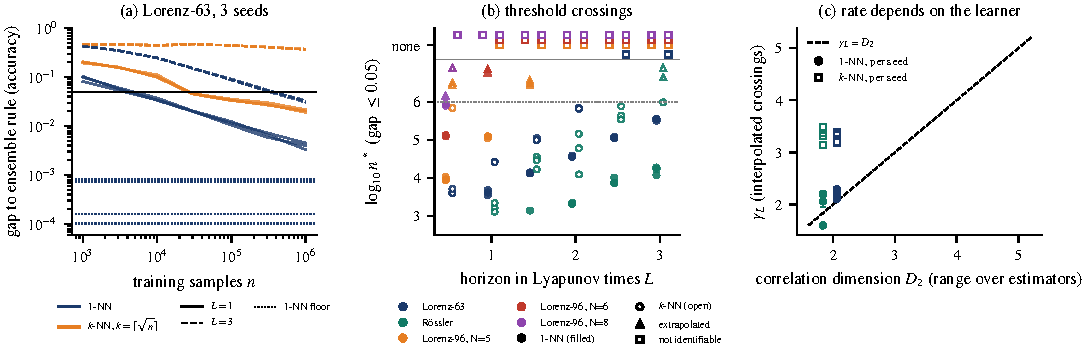
\includegraphics[width=\textwidth]{figs/fig_law3.pdf}
\caption{Learnability--horizon curves (exploratory). (a)~Lorenz-63: accuracy gap to the ensemble rule for 1-NN (blue) and $k$-NN (orange) at $L=1$ and $3$, three seeds each; dotted: estimated 1-NN floors. (b)~Sample size at which the gap reaches $0.05$, by system and learner; circle interpolated, triangle extrapolated from a floor fit (capped at $10^{6.9}$); dotted line: largest $n$ measured; row ``none'': no crossing (open square: not identifiable), offset by system. (c)~Per-seed growth rates from interpolated crossings against the range of correlation-dimension estimates; dashed: $\gamma_L=D_2$.}
\label{fig:law3}
\end{figure*}

\begin{table*}[!t]
\caption{Learnability--Horizon Rates for Two Learners (Gap $0.05$; Three Seeds)}
\label{tab:law3}
\centering
\footnotesize
\begin{tabular}{@{}lccccccc@{}}
\toprule
System & $\lambda$ & $D_2$ range & max 1-NN floor & $\gamma_L$, 1-NN & $\gamma_L$, $k$-NN & crossings 1-NN & crossings $k$-NN\\
\midrule
\csname @@input\endcsname gen/tab_law3.tex
\bottomrule
\end{tabular}
\vspace{2pt}

\parbox{\textwidth}{\footnotesize $\gamma_L$: mean $\pm$ s.d.\ over seeds of the slope of $\ln n^*$ on horizon (Lyapunov times), interpolated crossings only (seeds with $\ge3$ interpolated crossings in parentheses). Crossings: counts over 3 seeds $\times$ 6 horizons as interpolated/extrapolated/unattainable/not identifiable; the remainder were within tolerance at $n=10^3$. $^\ddagger$Exploratory only.}
\end{table*}

\subsection{Informational limits: what nine forecasting tasks achieve}\label{sec:res-atlas}
Real forecasting problems have no known ceiling; what can be measured is achieved skill, the information a fitted model extracts beyond the base rate, together with its model term (Eq.~\eqref{eq:lss}). Table~\ref{tab:atlas} and Fig.~\ref{fig:atlas} report it for nine tasks under strict walk-forward evaluation, with entity, time-block and two-way intervals; the two-way interval, which accounts for both sources of dependence, is primary, and every task except stock direction remains above zero under it.

\emph{Physical systems with good measurements gave the highest achieved skill.} Rain tomorrow with an NWP forecast as input reaches skill $\nwpNestBLSS$; the NWP benchmark alone achieves $\nwpBenchLSS$, about $\nwpRatio$ times the best model built from station observations on the same rows. Most of the achieved skill came from information that a physical model assembles and a station history lacks; this is consistent with a large epistemic term for station-only models, though the ceiling itself is unknown.

\emph{Tested models of social outcomes achieved modest skill; aggregated information achieved more.} Football home wins reach $\fbNestLSS$ from observable history, and closing betting odds ($\fbBenchLSS$) exceed every model we fitted. Presidential state outcomes reach $\prNestLSS$, but with only $\prTBn$ elections the time-block interval is wide ($\prTBlo$ to $\prTBhi$).

\emph{High accuracy is not high knowledge.} House seats are called correctly $\hsAcc$ of the time, which sounds like strong prediction; ``the incumbent party holds'' already scores $\hsAccZero$, and no model beats it in accuracy. This is the base-rate neglect of~\cite{kahneman1973psychology} in quantitative form: accuracy without a reference says nothing about what was known.

\emph{The tested market models extract almost nothing.} Next-day direction of large U.S.\ stocks and funds has skill $\stLSS$ under the entity bootstrap and an interval of $\stTBlo$ to $\stTBhi$ under time-block resampling, consistent with efficient-market theory for public price information~\cite{fama1970efficient}. The tested models extracted no reliably positive skill from the public price history under time-block resampling. This does not establish that the price history contains no information, since the ceiling is unknown, and says nothing about richer information sets.

\emph{Induction mostly holds forward.} Every task except stocks retains positive skill when every forecast is made strictly before its outcome, with a base rate that is itself point in time. Some nested increments are negative (adding entity history to rain, House and stock models made them slightly worse), a reminder that unused flexibility is a cost, not a neutral addition. Earthquakes show where skill comes from: in seismically active cells, recent activity (event counts over the past week, month and year, days since the last event, recent large shocks and activity in neighbouring cells) gives skill $\eqActiveModLSS$ over the base rate, while the entity model adds nothing ($\eqActiveEBLSS$); in quiet cells skill is $\eqQuietModLSS$. What is forecastable here is the clustering of events after recent activity.

\begin{figure}[!t]
\centering
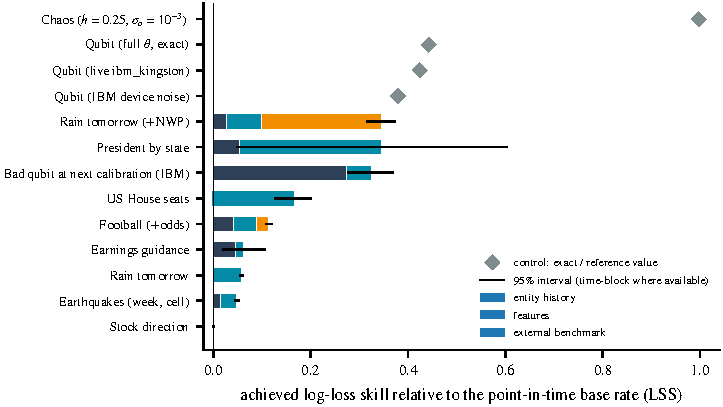
\includegraphics[width=\columnwidth]{figs/fig_atlas_rev.pdf}
\caption{Achieved log-loss skill relative to point-in-time base rates (primary nested model; stacked by achieved score improvement from entity history, features and external benchmarks; negative increments drawn to the left). Grey diamonds are reference values of controls (exact or simulated), not fitted skill. Bars: $95\%$ two-way (entity $\times$ time) intervals; dashed: qubit-only interval for the hardware task.}
\label{fig:atlas}
\end{figure}

\begin{table*}[!t]
\caption{Achieved Skill Relative to Point-in-Time Base Rates}
\label{tab:atlas}
\centering
\scriptsize
\setlength{\tabcolsep}{2.8pt}
\begin{tabular}{@{}lrcccccccccc@{}}
\toprule
Task & $n$ & $A_0$ & $A$ & $S_{acc}$ & LSS [entity CI] & [time CI] & [two-way CI] & entity & features & bench. & $\tau$\\
\midrule
\csname @@input\endcsname gen/tab_atlas_tb.tex
\bottomrule
\end{tabular}
\vspace{2pt}

\parbox{\textwidth}{\footnotesize $A_0$: base-rate accuracy; $S_{acc}$: accuracy skill over the base rate. LSS: achieved skill of the primary nested model; entity, features, bench.: achieved score improvements of nested models as shares of the baseline loss (signed; not mutual informations). Time CI: bootstrap over contiguous calendar blocks. Two-way CI: entities and time blocks resampled together (pigeonhole bootstrap~\cite{owen2007pigeonhole}), the primary interval. $^\S$Only qubit resampling is available for the hardware task; it ignores shared device-time shocks and its coverage is not validated. The Hellman--Raviv plug-in diagnostic reported in earlier versions (no coverage guarantee) is in the release. Controls report exact or ensemble reference values.}
\end{table*}

\subsection{Self-inflicted limits: when measured edge is illusory}\label{sec:res-self}
The measurement term of Proposition~\ref{prop:anat} is the one forecasters control and most often ignore. For two fixed decision rules $f,g$ with true accuracy difference $\Delta$, the difference $\tilde\Delta$ measured against recorded labels satisfies the exact identity $\tilde\Delta-\Delta=2\,\E[(f(X)-g(X))(\tilde q(X)-q(X))]$, where $q$ and $\tilde q$ are the true and recorded label probabilities (Proposition~\ref{prop:appinfl}). Errors that flip labels independently of everything only shrink an edge, by the factor $1-2\rho$; errors attached to particular entities and repeated over time can create one, and can turn a negative true edge into a positive measured one (Proposition~\ref{prop:apprev}). Because future labels carry the same errors, walk-forward validation rewards a model that learns them (Proposition~\ref{prop:appwf}). Validation in time order, the standard answer to Hume's problem in forecasting practice, does not protect against this.

The cheapest defence is to check labels only where it matters. Only rows on which two rules disagree affect the measured difference; checking a random sample of them bounds the true edge on the evaluated population with an exact hypergeometric guarantee (Proposition~\ref{prop:appaudit}).

The mechanism was found in the model that motivated this work: a forecast of whether a firm's diluted earnings beat the midpoint of its original guidance~\cite{ciconte2014midpoint}. The $\ecRem$ rows later removed because their labels had been extracted wrongly (continuing-operations guidance scored against total earnings, quarters mismatched) carried an apparent edge of $\ecRemEdge$ points over the base rate. On a fixed cohort of $\ecRows$ correctly labelled forecasts, the edge was $\ecA$ points ($\ecAlo$ to $\ecAhi$) before and $\ecB$ ($\ecBlo$ to $\ecBhi$) after retraining on cleaned history, a paired change of $\ecDiff$ ($\ecDifflo$ to $\ecDiffhi$): no effect of retraining was detected. An audit of 40 randomly drawn rows from the $\auND$ disagreement rows of the $\auPop$-row audit population, adjudicated by a single AI reviewer against a fixed checklist on the guidance side of each label, found $\eAuditE$ errors in 39 verifiable rows and one unresolvable row; counting that row as potentially wrong, the weighted edge on that population is bounded below by $\auLBwHb$ points ($\auLBwHa$ if it is excluded; Fig.~\ref{fig:illusory}), so the audit could not certify a positive edge; using the rows it verified as correct, the bound tightens to $\auTightB$ points. The guarantee covers sampling error only and assumes the verdicts are correct. Independent checks without AI judgement confirmed the reported-EPS side of $\xcEpsMatch$ of the $\xcN$ rows against SEC XBRL filings and left $\xcGuidFlagAI$ guidance verdicts unresolved; counting every unresolved row as wrong moves the bound to $\xcBallTight$ points, so a positive edge still cannot be certified. A lower bound below zero reflects weak evidence about the edge; it does not show that the true edge is negative. No human second adjudication has been done. The defensible conclusion is that the apparent advantage, almost three points before cleaning ($\eBeforeEdge$), was concentrated in invalid or target-incompatible evaluation rows and that no advantage was established on the retained cohort. Because the removed rows cannot be relabelled, the application does not demonstrate the sign reversal that the theory shows to be possible. The invalid rows recur within issuers: $\ibRecurRows$ of the $\ibInv$ belong to $\ibRecur$ issuers with invalid rows in two or more fiscal periods, and the entity rule matched their recorded outcomes on $\ibEbInv\%$ of invalid rows against $\ibBaseInv\%$ for the base rate, while on valid rows the two were close ($\ibEbVal\%$ and $\ibBaseVal\%$). The audit's hypergeometric step has exact coverage of at least $\covExactMin\%$, and Monte Carlo checks of the implemented bound are in Appendix~\ref{app:coverage}. The companion paper~\cite{abraham2026illusory} gives the full analysis, including the audit weights.

\begin{figure*}[!t]
\centering
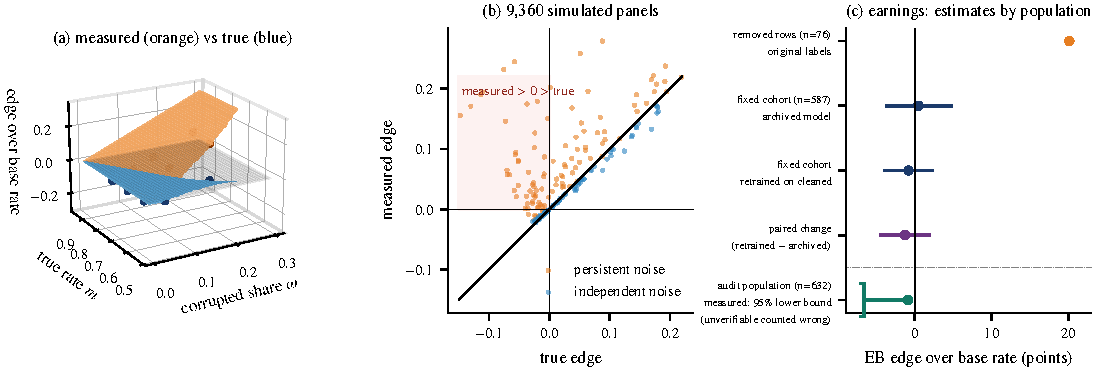
\includegraphics[width=\textwidth]{figs/fig_illusory.pdf}
\caption{Illusory edge. (a)~Measured (orange) and true (blue) edge of an entity rule over the base rate under persistent label corruption: surfaces from Proposition~\ref{prop:apprev}, points from simulation. (b)~Measured against true edge in 9{,}360 simulated panels. (c)~Earnings: each estimate labelled by its population (points; bars: 95\% issuer-bootstrap intervals): removed rows against their original labels, the fixed cohort before and after retraining and their paired change, and the audit population's measured weighted edge with its one-sided 95\% hypergeometric lower bound, counting the unverifiable row as wrong.}
\label{fig:illusory}
\end{figure*}

\subsection{Information versus computation: quantum classifiers}\label{sec:res-qc}
Proposition~\ref{prop:appqc} settles the theoretical question: a quantum model applied to classical inputs is, given its training data, a randomised function of those inputs, and cannot exceed their Bayes ceiling. It may approach the ceiling with less computation or, for constructed problems, fewer samples~\cite{liu2021rigorous,huang2021information}; whether it fits real forecasting data better is empirical. We compared variational circuits and quantum kernels with matched classical models (logistic regression, gradient boosting, a classical Fourier surrogate of the variational circuit and an RBF support-vector machine) on identical six-dimensional inputs in eight domains, selecting each family's model on validation data (Table~\ref{tab:quantum}).

No quantum model was significantly better than its classical counterpart in any domain (smallest Holm-adjusted $p=\qrevMinHolm$), and the classical model was better under both resampling schemes in $\qrevNsigWorse$. The one case that depends on the dependence model is stocks: the variational circuit (skill $\qrevStLq$) beat the selected classical model ($\qrevStLc$) under an entity bootstrap ($p=\qrevStPe$) but not under a month-block bootstrap ($p=\qrevStPt$); with shared market shocks the latter is the relevant one, and both skills are close to zero. This is a failure to detect an advantage in small simulated circuits, not proof that none exists. The decomposition explains why only this comparison is possible: quantum computation can act only on the model term, and because the real-task ceilings are unknown, the size of the remaining model term, and so the room for any model to improve, is not identified here.

\begin{table*}[!t]
\caption{Quantum and Classical Models Selected on Validation Data (Test LSS)}
\label{tab:quantum}
\centering
\scriptsize
\setlength{\tabcolsep}{3pt}
\begin{tabular}{@{}lrcccccccc@{}}
\toprule
Domain & $n_{\rm test}$ & selected classical & selected quantum & $\Delta$LL (Q$-$C) & 95\% CI, entity & 95\% CI, time & DM $p$ & boot.\ $p$ (entity / time) & Holm $p$\\
\midrule
\csname @@input\endcsname gen/tab_quantum_rev.tex
\bottomrule
\end{tabular}
\vspace{2pt}

\parbox{\textwidth}{\footnotesize Selection by validation log loss within each family on identical six-dimensional inputs; the variational circuits also use the validation split for early stopping. $\Delta$LL $>0$: quantum worse. Entity: bootstrap over entities; time: bootstrap over calendar months (20 contiguous blocks for the synthetic tasks, 6 election years for the House). DM $p$: one-sided Diebold--Mariano (quantum better), approximate under panel dependence. Boot.\ $p$: one-sided, share of bootstrap differences $\ge0$. Holm $p$: Holm adjustment over the eight domains of the larger of the two bootstrap $p$-values.}
\end{table*}

\subsection{Where quantum resources change what is knowable}\label{sec:res-side}
Quantum resources can change predictability by changing the information. In the CHSH game two players receive independent uniform bits $a,b$, answer $x,y$ without communicating and win if $x\oplus y=a\wedge b$; the best classical strategy wins with probability $0.75$, and a shared maximally entangled pair allows $\cos^2(\pi/8)\approx0.854$~\cite{clauser1969proposed,tsirelson1980quantum}. Each player is in effect predicting a function of the other's input and output, so the game measures how much a correlated system predicts about a distant event. The bound $0.75$ belongs to this game, not to prediction in general.

In simulation, the entangled strategy won $\chshSim$ of rounds. A forecaster predicting one qubit of a maximally entangled pair, measured in a basis chosen at random, is right half the time with no side information, $\sideCls$ of the time when holding the partner's computational-basis outcome recorded before the basis was chosen, and always ($\sideQ$) when holding the partner qubit itself and told the basis afterwards; this last case predicts the chosen measurement, not the outcomes of incompatible measurements simultaneously~\cite{berta2010uncertainty,konig2009operational}.

On IBM's ibm\_kingston on \liveDate, the game was won in $\liveChsh$ of $\liveTrials$ rounds (standard error $\liveChshSE$), above the classical $0.75$ and close to the quantum maximum; both qubits sit on one chip, so this demonstrates the game and is not a Bell test. In the loophole-free Delft experiment~\cite{hensen2016second}, reanalysed with its released selection code, the $\bellN$ valid trials give $S=\bellS\pm\bellSerr$ and a win rate of $\bellW$ ($\bellWlo$--$\bellWhi$) under the heralded-state convention of the original analysis; with the literal winning condition the rate is $\bellWlit$, which does not exceed $0.75$, and the published complete analysis reports $p=\bellP$. Predicting Bob's outcome from his own setting gives $\bellOwn$; adding Alice's setting and outcome gives $\bellSide$ ($\bellSidelo$--$\bellSidehi$). Entanglement, not computation, is the quantum resource that moves a predictability limit, and in the loophole-free experiment reanalysed here the gain is real but small and statistically modest (Fig.~\ref{fig:hardware}).

\begin{figure*}[!t]
\centering
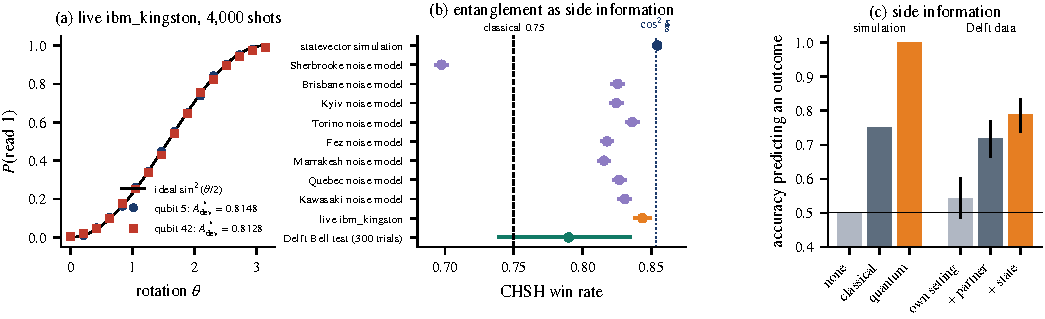
\includegraphics[width=\textwidth]{figs/fig_hardware.pdf}
\caption{Quantum hardware. (a)~Live ibm\_kingston: measured $P(\text{read }1)$ after $R_y(\theta)$ for two qubits, 4{,}000 shots per point, with the ideal response. (b)~CHSH win probability in simulation, on eight IBM device noise models, on ibm\_kingston (a single-chip game, not a Bell test) and in the Delft loophole-free Bell test (heralded-state winning condition). (c)~Accuracy of predicting an outcome with and without side information.}
\label{fig:hardware}
\end{figure*}

\subsection{Forecasting the forecasting machine}\label{sec:res-drift}
Quantum processors are themselves physical systems whose future can be forecast. IBM recalibrates its processors roughly daily; using $\drObs$ calibration records of $\drQubits$ qubits on three processors over $\drDays$ days~\cite{norton2026drift}, deduplicated on the calibration timestamp, we forecast each qubit's next calibration walk-forward. Readout and two-qubit gate errors are partly forecastable one calibration ahead (mean-squared-error skill $\drRoOne$ and $\drCzOne$ against each qubit's own history), decaying to $\drRoFt$ and $\drCzFt$ two weeks ahead. Coherence times are at most weakly forecastable ($T_1$: $\drToneOne$ [$\drToneOnelo$, $\drToneOnehi$]; $T_2$: $\drTtwoOne$), consistent with fluctuations driven by microscopic defects~\cite{klimov2018fluctuations,carroll2022dynamics}. Whether a qubit will be out of tolerance at its next calibration (base rate $\dbPBase$) is forecast with skill $\dbPHgbLSS$ ($\dbPHgbLSSlo$--$\dbPHgbLSShi$); a qubit that was bad is out of tolerance next time with probability $\dbPBadBad$, against $\dbPBadGood$ after a good calibration (Figs.~\ref{fig:drift},~\ref{fig:heat}). Intervals resample qubits and ignore shared device-time shocks, so their coverage is not validated; an independently collected dataset over $\drSecDays$ days shows the same pattern. The same machines that cannot raise a classical ceiling have parts that the tested models forecast and parts they did not. The split is consistent with prior work attributing coherence-time fluctuations to microscopic defects~\cite{klimov2018fluctuations,carroll2022dynamics}, but the experiment establishes only differences in forecast performance, not their mechanism, and weak performance of the tested coherence-time models does not rule out exploitable persistence.

\begin{figure*}[!t]
\centering
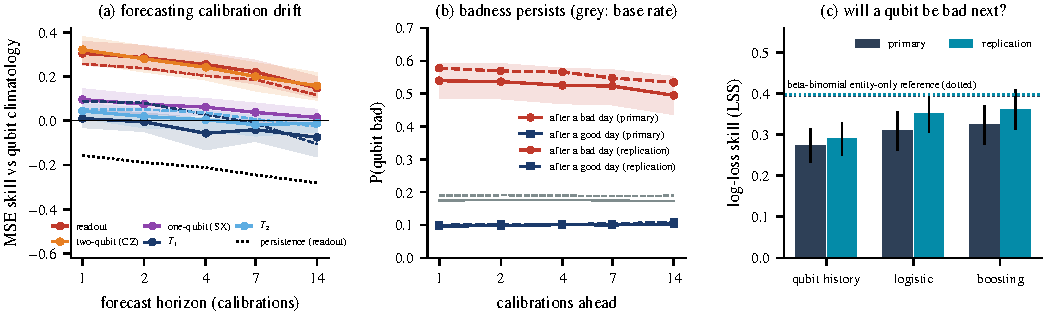
\includegraphics[width=\textwidth]{figs/fig_drift.pdf}
\caption{Forecasting IBM processor calibrations. (a)~Mean-squared-error skill against each qubit's climatology by horizon (bands: 95\% qubit-clustered intervals; dashed: replication dataset; dotted: persistence for readout error). (b)~Probability that a qubit is out of tolerance $k$ calibrations after a bad (red) or good (blue) calibration; grey: base rate. (c)~Log-loss skill of three models for the out-of-tolerance task; dotted: beta-binomial entity-only reference.}
\label{fig:drift}
\end{figure*}

\begin{figure*}[!t]
\centering
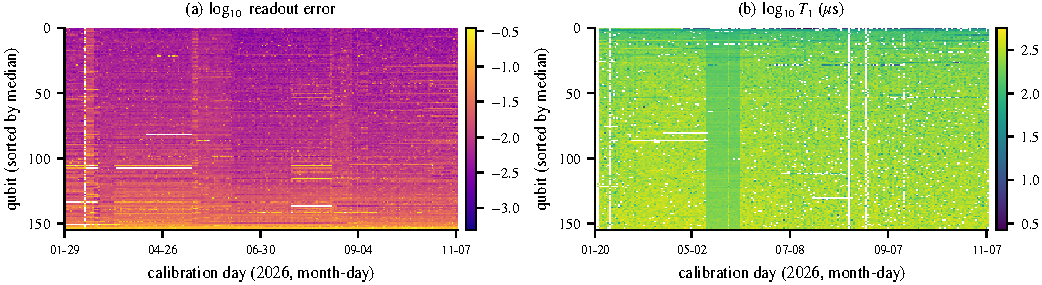
\includegraphics[width=\textwidth]{figs/fig_drift_heat.pdf}
\caption{Calibration histories of ibm\_kingston: (a)~readout error and (b)~$T_1$ for each qubit (rows, sorted by median) at each daily calibration (columns), January--November 2026. Three-dimensional renderings are in Appendix~\ref{app:render}.}
\label{fig:heat}
\end{figure*}

\subsection{Falsifiable predictions: the preregistration scorecard}\label{sec:res-prereg}
H1 has two components: H1a (the best learner within $0.02$ of the qubit ceiling at $n\ge10^4$) was met; H1b (the Cover--Hart plug-in at or above the reference in at least 80\% of control settings) failed ($\chValidPct\%$). For H2, the rank correlation between predicted and measured skill was $\preRho$, above the preregistered $0.6$, but only $\preHits$ of $\preN$ point intervals contained the measured value, and the misses were mostly toward lower skill: we expected more of the future to be knowable than it was. H3 (accuracy skill below $0.15$ for earnings and stocks) and H6 (the chaos ceiling approaching one as noise falls, the qubit ceiling fixed) were consistent with the data. For H4 the simulation component was met and the earnings edge fell after cleaning, though the fixed-cohort analysis attributes the fall to removed rows more than to retraining. For H5 no significant quantum advantage was detected; failing to reject is not evidence of absence. Analyses added after the preregistration, including all hardware, Bell-test and multi-system chaos results, are exploratory.

\section{Discussion: How Much of the Future Is Knowable?}\label{sec:discussion}
The question has a measured answer for each event and information set, not a single one. The results nonetheless show a pattern.

\emph{Where the limit is epistemic, it moves with measurement.} In a deterministic chaotic system the ensemble forecast's accuracy approaches one as precision improves, but each tenfold gain buys a fixed increment of horizon, and learning the dynamics from data costs a factor of roughly $\mathrm{e}^{2}$ to $\mathrm{e}^{3}$ more examples per Lyapunov time for the learners we tested. Laplace was right about such systems in principle and wrong about them in practice. Weather shows a similar pattern in practice: the NWP benchmark alone achieved $\nwpBenchLSS$ of the combined model's $\nwpNestBLSS$, against $\nwpBestObs$ for the best observation-only model.

\emph{Where the limit is ontic under the stated model, more knowledge of the preparation does not move it.} Under the Born rule, exact knowledge of the preparation leaves more than half of the outcome's entropy unremoved, and the hardware channels we fitted only subtracted from the ceiling. The one way around it is to change what is known about the outcome, by holding an entangled partner; computation on classical data does not.

\emph{Where achieved skill is modest, others often hold the information.} In social and economic tasks the tested models extracted modest skill, and the benchmarks that aggregate other people's information (weather models, betting odds) carried most of the achieved skill. From public market prices, the tested models extracted no reliably positive skill about tomorrow's direction; the ceilings of these tasks remain unknown.

\emph{The limit forecasters most often exceed is the one they impose on themselves.} The largest apparent edge in this study, in the earnings model, sat in evaluation rows with persistent label errors that standard validation could not see. The House result shows the same overstatement in a different guise: accuracy against no reference. Our own preregistered intervals erred toward optimism. In the cases studied here, claimed or expected skill exceeded achieved skill; because the real-task ceilings are unknown, we cannot say how far achieved skill falls short of what is knowable.

\emph{Implications.} For machine-learning forecasting, the decomposition says where effort pays: better information reduces the epistemic term, better models only the model term, and label audits the measurement term, which can dominate. For finance, near-zero skill in public prices is a measured property of one information set, not a statement about all of them. For quantum computing, faster or larger quantum models cannot raise a classical ceiling; quantum information changes predictability only when the information itself is quantum, and the hardware that would do this is a forecasting problem in its own right.

\emph{Scope.} The domains are a convenience sample of tasks with free data, and achieved skill measures predictive performance; interpreting it as a bound on knowability requires additional assumptions about the baseline and the forecasting distribution. The chaos and hardware studies are exploratory, and each could support a dedicated study.

\section{Threats to Validity}\label{sec:threats}
\emph{Ceilings.} Real-task ceilings are unknown; achieved skill depends on models and features, and nearest-neighbour plug-in values are diagnostics, not bounds. \emph{Chaos.} The ensemble reference is an approximate posterior validated for Lorenz-63 at larger noise and horizons up to two Lyapunov times; chaos results are gaps to that reference; two learners, one relative noise level and three seeds per system in the tables and twenty in the uncertainty analysis, which does not include reference error were used. \emph{Labels.} Earnings labels are machine-extracted, the audit covers only disagreement rows, adjudicated by one AI reviewer without independent second adjudication, and the removed rows could not be relabelled. \emph{Dependence.} Two-way entity-by-time intervals are used for achieved skill, but they treat time blocks as exchangeable, and the hardware and quantum comparisons use one-way resampling only. \emph{Data.} Revised observations and catalogues, survivorship in the stock universe, guidance revisions and calibration publication delays are unresolved point-in-time risks; House data end in 2018; the NWP benchmark is a calibrated proxy over 17 months. \emph{Hardware.} One processor on one day for the live run, a single-chip game rather than a Bell test, third-party calibration polling, qubit-resampled intervals that ignore shared device-time shocks. \emph{Preregistration.} Timing rests on local records; many analyses are exploratory.

\section{Conclusion}
How much of the future is knowable is a quantity, not a slogan. It is the Bayes ceiling of a stated information set, and the measured loss of any forecast splits exactly into randomness irreducible under a stated physical model, information not used, imperfect use of the information held, and a signed distortion from errors in the record. Under quantum theory, a qubit's outcome stays partly unknowable however well it is prepared; a chaotic flow becomes knowable as measurement sharpens, but each extra unit of horizon costs exponentially in precision and, for the learners we tested, steeply in data; the tested models of real social and economic outcomes achieved modest skill, mostly through information that experts and physical models already aggregate; and the largest apparent edge we found sat in rows with persistent label errors. Quantum computers do not raise these ceilings; quantum entanglement changes them by changing the information, and in the loophole-free experiment reanalysed here the gain is real but small. The future is partly knowable; the controls show by how much, the real tasks show what tested models achieve, and in the cases studied the claims exceeded the achievement.

\appendices
\begin{figure*}[!t]
\centering
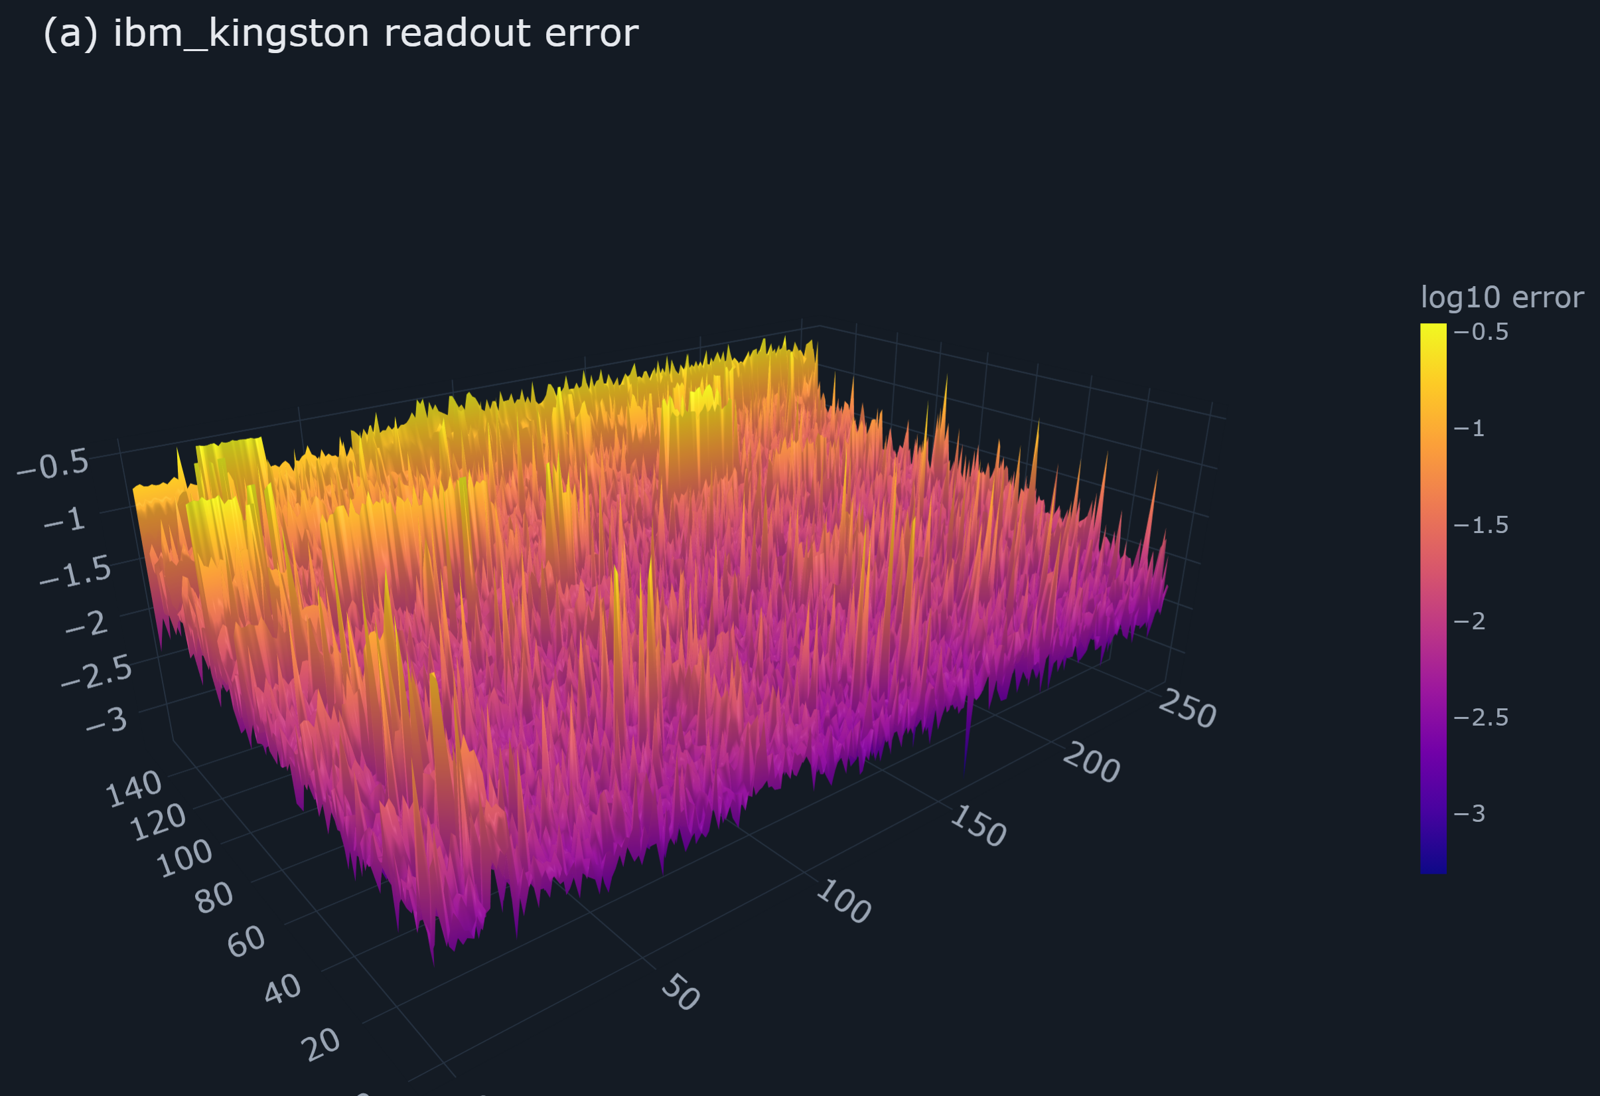
\includegraphics[width=0.53\textwidth]{figs/comp_drift3d_readout.png}\hfill
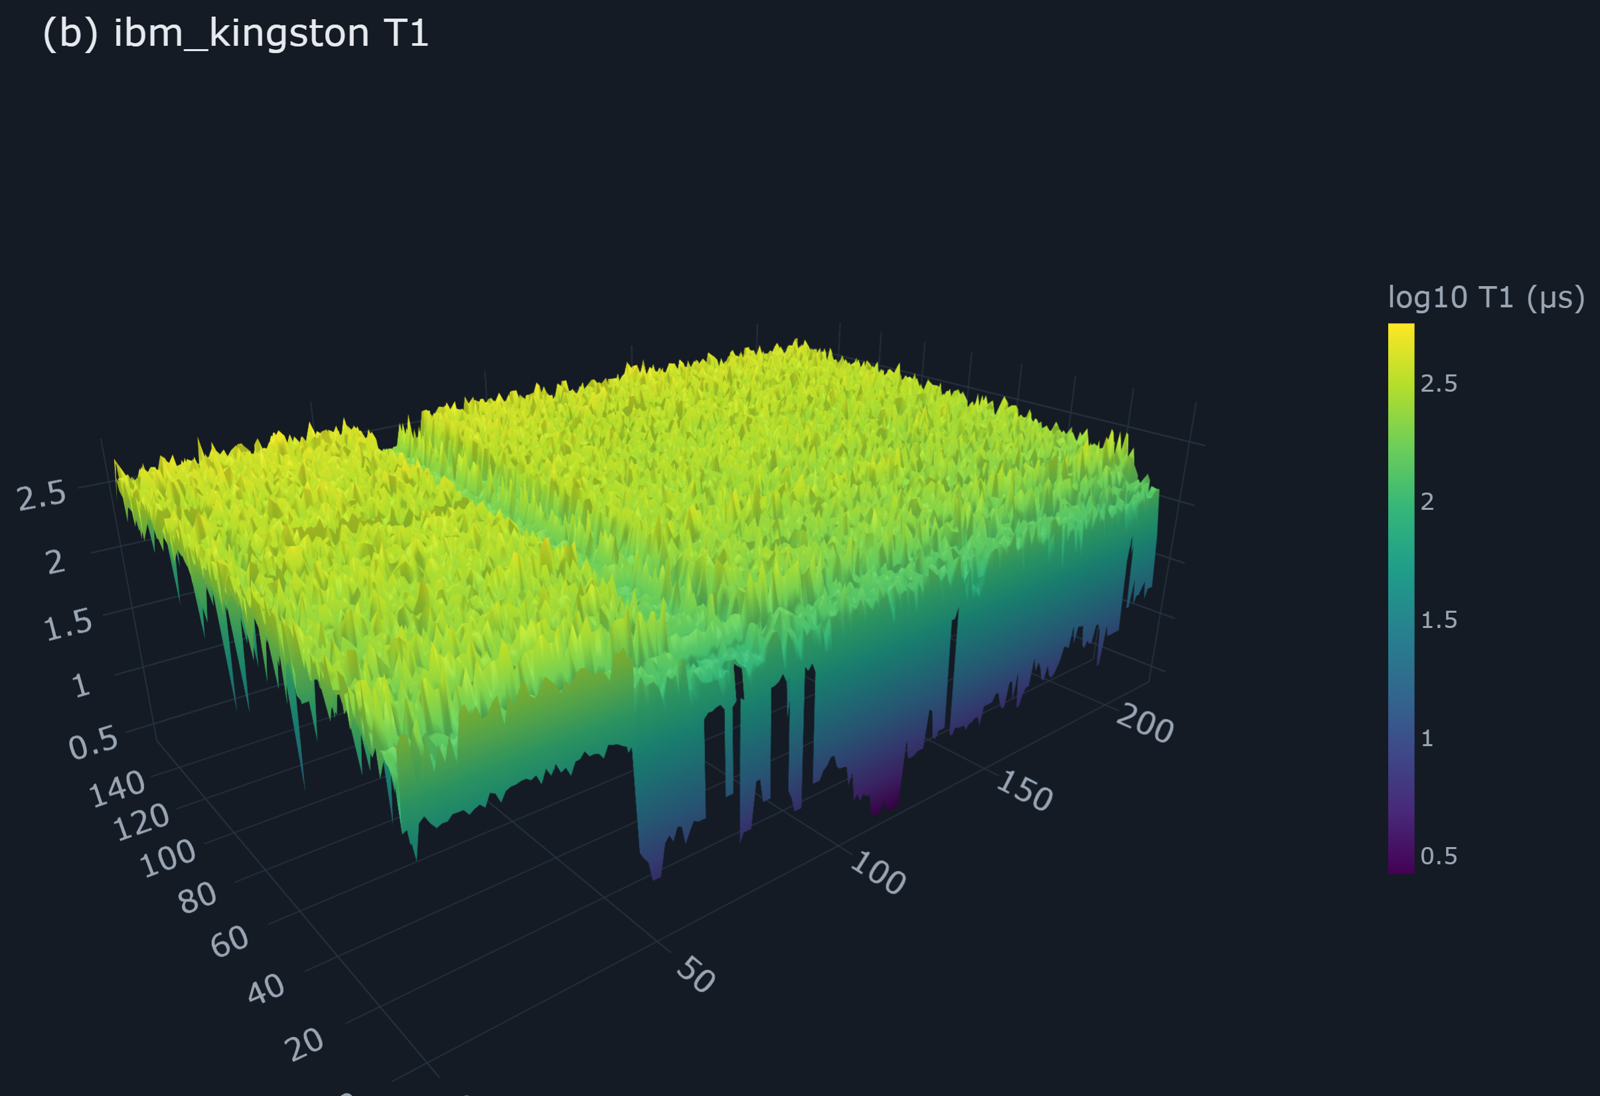
\includegraphics[width=0.46\textwidth]{figs/comp_drift3d_t1.png}\\[3pt]
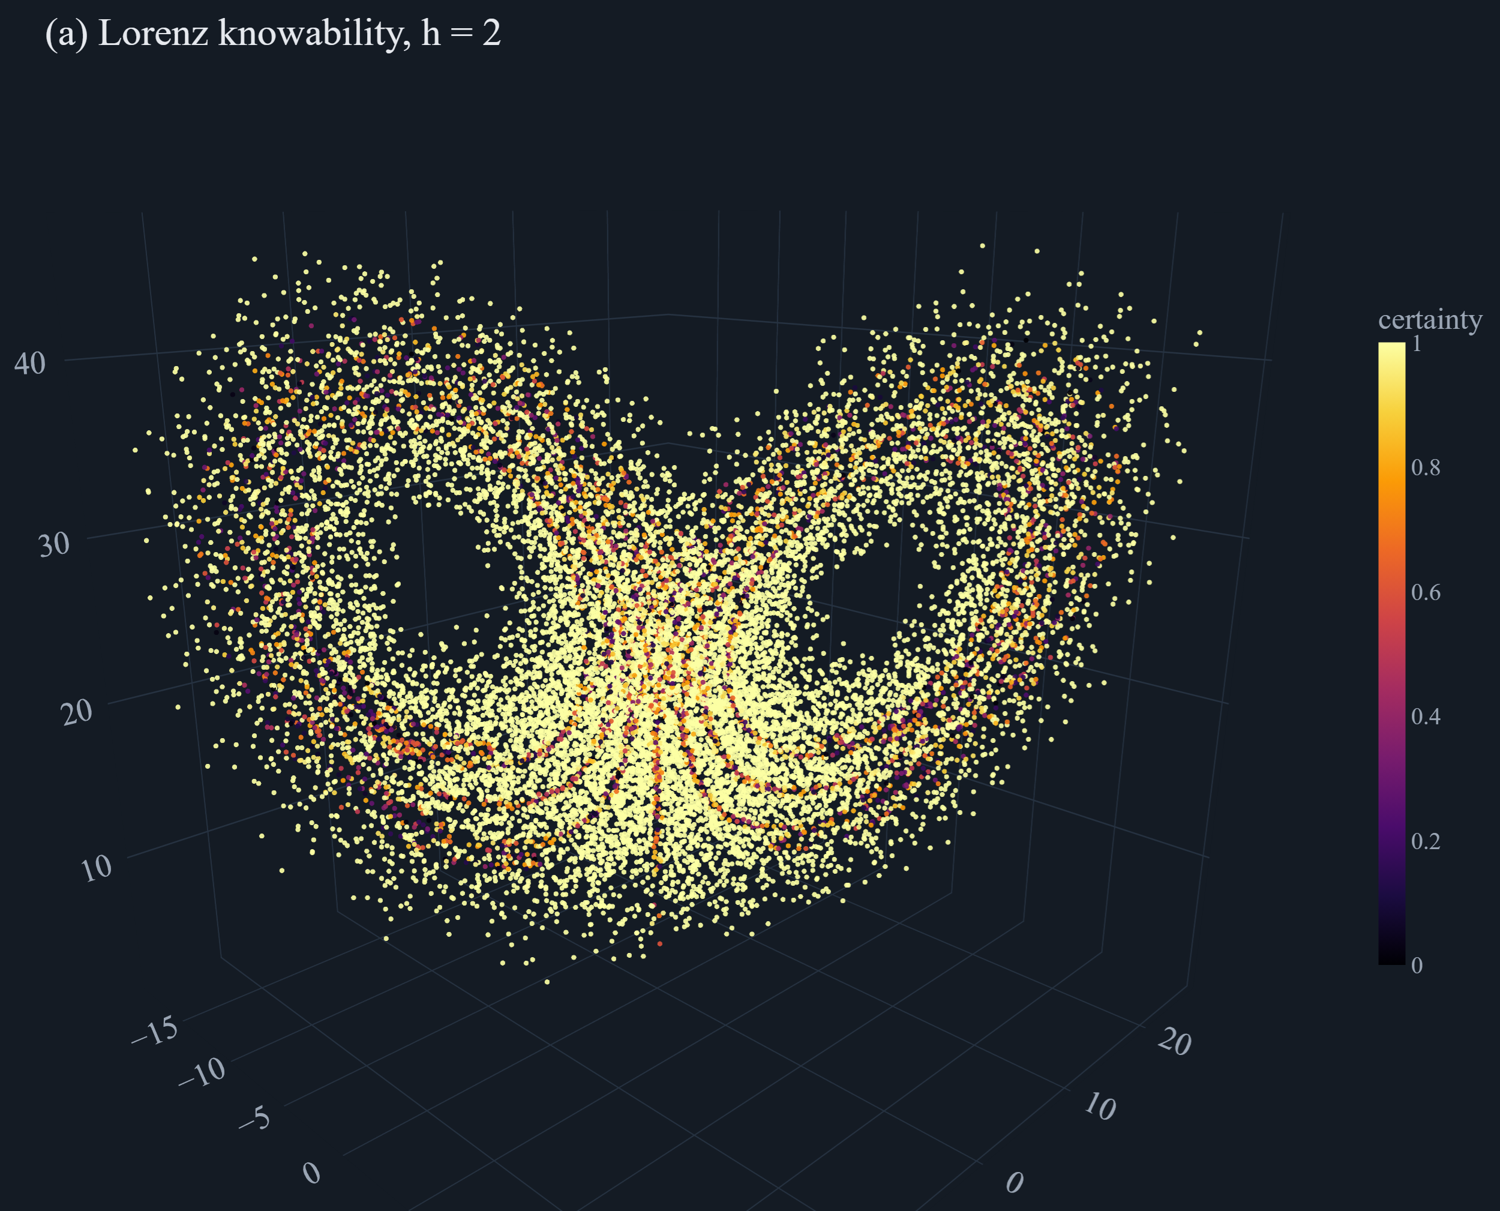
\includegraphics[width=0.6\textwidth]{figs/comp_lorenz_h2.png}
\caption{Renderings from the interactive companion. Top: ibm\_kingston calibration surfaces of Fig.~\ref{fig:heat}, $\log_{10}$ readout error and $\log_{10}T_1$ ($\mu$s) over qubit (depth, sorted by median) and calibration day (horizontal). Bottom: ensemble certainty $2|\hat\eta-\tfrac12|$ of the sign of $x(t+2)$ on the Lorenz attractor ($\sigma_o=0.1$).}
\label{fig:render}
\end{figure*}
\section{Definitions, Assumptions and Proofs}\label{app:math}
Throughout, $(X,Y)$ is a test example drawn from a stated evaluation distribution $P$ on $\mathcal X\times\{0,1\}$, where $X$ collects every quantity available at the decision time (the information set $\F$ is the $\sigma$-algebra generated by $X$). We assume $0<P(Y=1)<1$, so that $H(Y)>0$, and write $\eta(x)=P(Y=1\mid X=x)$ for a fixed version of the regression function, $r(x)=\min\{\eta(x),1-\eta(x)\}$, and $\Hb$ for the binary entropy in nats. For forecasting problems the training history is part of the setting and is never part of $X$ unless stated; temporal dependence and drift are discussed in Section~\ref{sec:design}.

\subsection{Ceilings and learnability}
\begin{definition}[Bayes ceiling relative to $\F$]
$A^*(\F)=\E\max\{\eta(X),1-\eta(X)\}=1-\E\,r(X)$ and $\mathrm{LL}^*(\F)=H(Y\mid X)=\E\,\Hb(\eta(X))$.
\end{definition}
\begin{definition}[Algorithm-specific learnability]
Let $\mathcal A$ map a training sample $S_n=((X_i,Y_i))_{i\le n}$ to a (possibly randomized) classifier. With $S_n\sim P^n$ independent of $(X,Y)\sim P$,
\begin{gather*}
A_n(\mathcal A;P)=\E_{S_n}\Pr_{(X,Y),\,\xi}\{\mathcal A(S_n)(X;\xi)=Y\},\\
G_n(\mathcal A;P)=A^*(\F)-A_n(\mathcal A;P),
\end{gather*}
where $\xi$ is internal randomness independent of $(S_n,X,Y)$. No optimization over algorithms is implied; every finite-sample statement in this paper concerns a named algorithm. $\mathcal A$ is \emph{Bayes consistent} for $P$ if $G_n\to0$.
\end{definition}
\begin{definition}[Knowable fraction]
$\kappa(\F)=I(Y;X)/H(Y)=1-H(Y\mid X)/H(Y)\in[0,1]$, the uncertainty coefficient of~\cite{theil1970estimation} applied to the decision-time information.
\end{definition}

\begin{lemma}[Ceiling]\label{lem:app1}
Let $q:\mathcal X\to[0,1]$ be measurable and let $\hat Y\mid X\sim\mathrm{Bernoulli}(q(X))$ with the randomization independent of $Y$ given $X$. Then $P(\hat Y=Y)\le A^*(\F)$. If $\hat p:\mathcal X\to(0,1)$ is measurable, $\E[-\log\hat p(X)^{Y}(1-\hat p(X))^{1-Y}]=H(Y\mid X)+\E\,\KL(\eta(X)\Vert\hat p(X))$.
\end{lemma}
\begin{proof}
By conditional independence, $P(\hat Y=Y\mid X)=q\eta+(1-q)(1-\eta)\le\max(\eta,1-\eta)$ almost surely; take expectations. The second identity is the decomposition of the cross-entropy given $X$, integrated over $X$.
\end{proof}
A classifier trained on $S_n$ satisfies the lemma conditionally on $S_n$ when the test example is independent of $S_n$; hence $A_n(\mathcal A;P)\le A^*(\F)$ for every $n$.

\emph{Nearest neighbours.} If $\eta$ is continuous and $X$ has a density on a separable metric space, the 1-NN error converges to $R_{\rm NN}=\E[2r(X)(1-r(X))]$~\cite{cover1967nearest}, so the asymptotic excess error of 1-NN is $\E[r(1-2r)]\ge0$, with equality only if $r\in\{0,\tfrac12\}$ almost surely. The $k$-NN rule with $k_n\to\infty$ and $k_n/n\to0$ is universally consistent~\cite{stone1977consistent}. Inverting $R_{\rm NN}\le2R^*(1-R^*)$ gives $R^*\ge\tfrac12(1-\sqrt{1-2R_{\rm NN}})$ for the \emph{population} $R_{\rm NN}\le\tfrac12$; substituting a finite-sample error estimate yields an asymptotic plug-in diagnostic without coverage guarantee, and it is undefined when the estimate exceeds $\tfrac12$. The Hellman--Raviv inequality $R^*\le\tfrac12H_2(Y\mid X)$ (bits)~\cite{hellman1970probability} likewise yields only a plug-in diagnostic $\kappa_U$ when $R^*$ is replaced by such an estimate.

\emph{Log-loss skill.} For a forecast $\hat p$ and a baseline $p_0$ that is measurable with respect to a smaller information set $\F_0$,
\begin{equation*}
\LSS=1-\frac{\E\ell(\hat p)}{\E\ell(p_0)}=1-\frac{H(Y\mid X)+\E\,\KL(\eta\Vert\hat p)}{H(Y\mid \F_0)+\E\,\KL(\eta_0\Vert p_0)},
\end{equation*}
with $\eta_0=P(Y=1\mid\F_0)$. LSS therefore mixes the information gap $H(Y\mid\F_0)-H(Y\mid X)$ with the misspecification, estimation, calibration and drift losses $\E\,\KL$ of both forecasts; a small LSS does not imply a small $\kappa$, and LSS exceeds $1-H(Y\mid X)/H(Y\mid\F_0)$ whenever the baseline's divergence term is large. These are population (ratio-of-expectations) quantities. The empirical LSS is a ratio of test-set averages. It converges to the population ratio when test examples are i.i.d.\ draws from a fixed distribution, or under stationarity and ergodicity with a fixed forecast, but not in general under drift or strong dependence; its finite-sample expectation generally differs from the population ratio.

\subsection{Anatomy of forecast loss}
\begin{proposition}[Four-term decomposition]\label{prop:appanat}
Let $\F\subseteq\F_\infty$ be information sets generated by random elements $X$ and $(X,Z)$, let $\hat p$ be a forecast that is $\F$-measurable given the training data and takes values in $(0,1)$, and let all entropies and the expected log losses against $Y$ and $\tilde Y$ be finite (for example, $\hat p\in[\epsilon,1-\epsilon]$ for some $\epsilon>0$); all expectations are conditional on the training data. With $\eta_\F=P(Y=1\mid\F)$ and natural logarithms, the expected log loss against the true outcome is
\begin{equation*}
\E\,\ell(\hat p,Y)=\underbrace{H(Y\mid\F_\infty)}_{\text{ontic}}+\underbrace{I(Y;Z\mid X)}_{\text{epistemic}}+\underbrace{\E\,\KL(\eta_\F\Vert\hat p)}_{\text{model}}.
\end{equation*}
If the forecast is scored against a recorded label $\tilde Y$, then $\E\,\ell(\hat p,\tilde Y)=\E\,\ell(\hat p,Y)+M$ with $M=\E[(\tilde Y-Y)\ln\{(1-\hat p(X))/\hat p(X)\}]$, which can take either sign; equivalently, $\E\,\ell(\hat p,\tilde Y)=H(\tilde Y\mid\F)+\E\,\KL(\tilde\eta_\F\Vert\hat p)$ with $\tilde\eta_\F=P(\tilde Y=1\mid\F)$.
\end{proposition}
\begin{proof}
Conditionally on $X$, $\E[-\ln\hat p(Y)\mid X]=\Hb(\eta_\F(X))+\KL(\eta_\F(X)\Vert\hat p(X))$ by adding and subtracting $\E[\ln\eta_\F(Y)\mid X]$; taking expectations gives $H(Y\mid\F)+\E\,\KL$. The chain rule gives $H(Y\mid X)=H(Y\mid X,Z)+I(Y;Z\mid X)$. For the measured loss, $\ell(p,\tilde y)-\ell(p,y)=-(\tilde y-y)\ln p+(\tilde y-y)\ln(1-p)=(\tilde y-y)\ln\{(1-p)/p\}$ for binary labels; taking expectations gives $M$, and the same steps as above with $\tilde Y$ give the second form. Conditioning on the training data throughout makes the statement hold for a trained model.
\end{proof}
Which part of $H(Y)$ is ``ontic'' depends on what $\F_\infty$ can contain. For a classical deterministic system observed exactly, $H(Y\mid\F_\infty)=0$. For a quantum measurement, quantum theory with the preparation in $\F_\infty$ gives $H(Y\mid\F_\infty)>0$. Bell tests exclude locally causal completions under their assumptions but do not show that every completion is indeterministic, so ``ontic'' here means irreducible under the stated quantum model and information access.

\subsection{Closed forms}
\begin{proposition}[Qubit]\label{prop:appqubit}
If $\theta\sim U(0,\pi)$ is known and $Y$ is the computational-basis outcome of $R_y(\theta)\lvert0\rangle$, then $A^*=\tfrac12+\tfrac1\pi$, $H(Y\mid\theta)=2\ln2-1$, $H(Y)=\ln2$ and $\kappa=1/\ln2-1$. Under the depolarizing channel $\rho\mapsto(1-p_{\rm d})\rho+p_{\rm d}I/2$, $A^*=\tfrac12+(1-p_{\rm d})/\pi$. Under readout errors $P(\text{read }1\mid0)=e_0$, $P(\text{read }0\mid1)=e_1$ with $\beta=1-e_0-e_1>0$, $a=(e_0-e_1)/2$ and $|2a|<\beta$, the Bayes rule thresholds $p'=e_0+\beta\sin^2(\theta/2)$ at $\tfrac12$ and
\begin{equation*}
A^*=\tfrac12+\tfrac1\pi\big[\beta\sin\theta_0+a(\pi-2\theta_0)\big],\qquad \cos\theta_0=2a/\beta,
\end{equation*}
which reduces to $\tfrac12+\beta/\pi$ only when $e_0=e_1$.
\end{proposition}
\begin{proof}
$p'-\tfrac12=a-\tfrac\beta2\cos\theta$, and for $\theta\sim U(0,\pi)$, $\E|a-b\cos\theta|=\pi^{-1}[2b\sin\theta_0+a(\pi-2\theta_0)]$ with $b=\beta/2$, $\cos\theta_0=a/b$, obtained by splitting the integral at $\theta_0$. The noiseless case is $a=0$, $\beta=1$; depolarizing gives $a=0$, $\beta=1-p_{\rm d}$. The entropy follows from the substitution $u=\cos\theta$: $\int_{-1}^1\Hb(\tfrac{1-u}2)\,\frac{du}{\pi\sqrt{1-u^2}}=2\ln2-1$, and $\E p=\tfrac12$.
\end{proof}

\begin{proposition}[Beta-binomial entity model]\label{prop:appbeta}
Assume exchangeable entities with rates $p_i\sim\mathrm{Beta}(\alpha,\beta)$, known hyperparameters, and outcomes conditionally i.i.d.\ Bernoulli$(p_i)$, and entity sample sizes independent of the rates (noninformative weighting), so that weighting entities by their number of outcomes leaves the rate distribution of the weighted population equal to $\mathrm{Beta}(\alpha,\beta)$. Then the oracle-rate accuracy is $A_1^*=\E[\max(p,1-p)]$ and its conditional entropy is $\E[H_2(p)]$, with $p\sim\mathrm{Beta}(\alpha,\beta)$. After a history of $n$ outcomes with $k$ successes the predictive probability is $m_k=(\alpha+k)/(\alpha+\beta+n)$, and the finite-history Bayes accuracy is
\[
A_1^*(n)=\sum_{k=0}^{n}\binom{n}{k}\frac{B(\alpha+k,\beta+n-k)}{B(\alpha,\beta)}\max(m_k,1-m_k).
\]
$A_1^*(n)$ is nondecreasing in $n$ and converges to $A_1^*$.
\end{proposition}
\begin{proof}
The closed forms follow from Beta--Bernoulli conjugacy: the posterior after $(n,k)$ is $\mathrm{Beta}(\alpha+k,\beta+n-k)$ and $k$ is beta-binomial. Monotonicity holds because the history of length $n$ is a function of the history of length $n+1$, so the Bayes accuracy of the larger $\sigma$-algebra is at least as large; convergence follows from posterior consistency for each $p_i\neq\tfrac12$ and dominated convergence.
\end{proof}
\emph{General rate law.} If sample sizes depend on the rates, the outcome-weighted population has some rate law $G$ that need not be Beta, and the conjugate formulas above no longer apply. The oracle quantities remain $A_1^*=\E_G[\max(p,1-p)]$ and $\E_G[H_2(p)]$, but the predictive probability must be derived from $G$: $m_k=\int p^{k+1}(1-p)^{n-k}\,dG(p)\big/\int p^{k}(1-p)^{n-k}\,dG(p)$, and $A_1^*(n)=\sum_{k}\binom nk\int p^k(1-p)^{n-k}\,dG(p)\,\max(m_k,1-m_k)$. Monotonicity in $n$ holds by the same argument, and convergence to $A_1^*$ follows from martingale convergence of $m_k$ to $p$.

Applied to real data, $(\alpha,\beta)$ are method-of-moments estimates and the model is an approximation; the resulting ceilings are model-based, not identified upper bounds.

\subsection{Label noise}
Let $\tilde Y$ be the recorded label and $\tilde q(x)=P(\tilde Y=1\mid X=x)$, $q=\eta$. All statements in this subsection concern \emph{fixed} decision rules $f,g:\mathcal X\to\{0,1\}$ evaluated under clean and corrupted labels; they do not describe pipelines retrained on corrupted labels unless stated.
\begin{proposition}[Inflation identity]\label{prop:appinfl}
$\tilde\Delta-\Delta=2\,\E[(f(X)-g(X))(\tilde q(X)-q(X))]$, where $\Delta=P(f=Y)-P(g=Y)$ and $\tilde\Delta$ uses $\tilde Y$.
\end{proposition}
\begin{proof}
$P(f=\tilde Y\mid X)-P(f=Y\mid X)=(2f-1)(\tilde q-q)$; subtract the same expression for $g$ and integrate.
\end{proof}
The main-text form follows when $X$ includes the entity and $f$ is constant within entities, with entities weighted by their share of outcomes.
\begin{proposition}[Symmetric independent noise]\label{prop:appsym}
If $\tilde Y=Y\oplus N$ with $N\sim\mathrm{Bernoulli}(\rho)$, $\rho<\tfrac12$, independent of $(X,Y)$, then $\tilde\Delta=(1-2\rho)\Delta$ for fixed rules, and the Bayes rule for $\tilde Y$ equals the Bayes rule for $Y$; a Bayes-consistent learner trained on corrupted labels therefore converges to the clean Bayes rule.
\end{proposition}
\begin{proof}
$\tilde q-\tfrac12=(1-2\rho)(q-\tfrac12)$ and $\tilde q-q=\rho(1-2q)$; insert into Proposition~\ref{prop:appinfl}: $\tilde\Delta-\Delta=-2\rho\,\E[(f-g)(2q-1)]=-2\rho\Delta$.
\end{proof}
\begin{proposition}[Sign reversal]\label{prop:apprev}
Let $q\equiv m>\tfrac12$ and let a fraction $\omega$ of entities (by outcome share) have $\tilde q=0$, the rest $\tilde q=m$, with $(1-\omega)m>\tfrac12$. Let $g\equiv1$ (the base-rate rule, which remains the Bayes rule for the pooled corrupted labels) and let $f$ be the entity-wise Bayes rule for $\tilde Y$. Then $\tilde\Delta=\omega$ and $\Delta=-\omega(2m-1)$.
\end{proposition}
\begin{proof}
$f=0$ on corrupted entities and $1$ elsewhere; Proposition~\ref{prop:appinfl} gives $\tilde\Delta-\Delta=2\omega m$, and directly $\Delta=\omega[(1-m)-m]$.
\end{proof}
\begin{proposition}[Time-ordered validation]\label{prop:appwf}
Assume (i) for each entity, outcomes and corruption are i.i.d.\ over time with fixed $(q_i,\tilde q_i)$ and $\tilde q_i\neq\tfrac12$; (ii) every evaluated entity has a past history whose length tends to infinity; (iii) the entity rule is the majority of the entity's past recorded labels. Then the walk-forward decisions converge almost surely to $\ind\{\tilde q_i>\tfrac12\}$ and the walk-forward measured edge converges to the in-sample measured edge. If held-out entities are forecast with the pooled base-rate rule, their entity-specific edge is zero.
\end{proposition}
\begin{proof}
By the strong law of large numbers the empirical recorded rate converges to $\tilde q_i$, so the majority decision is eventually constant and equal to $\ind\{\tilde q_i>\tfrac12\}$ ($\tilde q_i\ne\tfrac12$ rules out ties). Future recorded labels have the same distribution, so the expected measured accuracy of the eventual decision is the in-sample value. The last claim holds by construction of the fallback; other fallbacks (e.g.\ feature models) need not have zero entity-specific edge.
\end{proof}
\begin{proposition}[Disagreement audit on a fixed population]\label{prop:appaudit}
Let a finite evaluation population of $N$ rows with nonnegative weights $w_j$ be fixed, together with the recorded labels and two fixed decision vectors, and let $D$ be the set of $N_D$ disagreement rows. (a) $\tilde\Delta-\Delta$ depends only on the wrong labels in $D$, and $|\tilde\Delta-\Delta|\le2\sum_{j\in D_{\rm wrong}}w_j/\sum_jw_j$. (b) If $n$ rows are drawn uniformly without replacement from $D$, each sampled row is adjudicated correctly, and $e$ are found wrong, let $K_U$ be the largest $K$ with $\Pr\{\mathrm{Hypergeom}(N_D,K,n)\le e\}>\alpha$. With probability at least $1-\alpha$ over the sampling, $|D_{\rm wrong}|\le K_U$, and therefore $\Delta\ge\tilde\Delta-2W_{(K_U)}/\sum_jw_j$, where $W_{(K)}$ is the sum of the $K$ largest weights in $D$; with equal weights the bound is $\tilde\Delta-2(N_D/N)(K_U/N_D)$.
\end{proposition}
\begin{proof}
(a) On rows outside $D$ both rules make the same decision, so a wrong label changes both accuracies equally. A wrong label on row $j\in D$ changes the weighted difference by $\pm2w_j/\sum w$. (b) For fixed $K$ the number of wrong rows in the sample is hypergeometric; the set $\{K:\Pr(X\le e\mid K)>\alpha\}$ is a one-sided $(1-\alpha)$ confidence set by the usual test inversion, since $\Pr(X\le e\mid K)$ is nonincreasing in $K$. The weight bound is the worst case over which $K_U$ rows are wrong.
\end{proof}
The statement bounds the clean-label edge $\Delta$ on the fixed evaluation population, starting from the recorded-label edge $\tilde\Delta$; the guarantee covers sampling error only, conditional on correct adjudication of the sampled rows, and says nothing about future predictive edge, which requires a separate sampling model for future cases. The binomial Clopper--Pearson bound is valid for sampling with replacement and conservative relative to (b) for sampling without replacement.

\subsection{Classical inputs and quantum models}
\begin{proposition}[Classical-input ceiling]\label{prop:appqc}
Let a model with parameters $\phi=\phi(S_n)$ fitted on training data encode a test input $x$ into a state $\rho_\phi(x)$, apply a measurement, and output $\hat Y$. If the test example is independent of $S_n$ and the measurement randomness is independent of $Y$ given $(X,S_n)$, then conditionally on $S_n$ the chain $Y\to X\to\hat Y$ is Markov, $I(Y;\hat Y\mid S_n)\le I(Y;X)$ and $P(\hat Y=Y)\le A^*(\F)$.
\end{proposition}
\begin{proof}
Given $S_n$, $\hat Y$ is a randomized function of $X$; apply Lemma~\ref{lem:app1} conditionally and the data-processing inequality, then average over $S_n$.
\end{proof}
The proposition excludes accuracy above the Bayes ceiling of the classical input; it permits a quantum model to approach that ceiling with less computation or, for structured $\eta$, fewer samples~\cite{liu2021rigorous,huang2021information}. It does not apply when the predictor holds a quantum system correlated with the predicted one, which is a different information set.

\section{Coverage Studies}\label{app:coverage}
\emph{Two-way intervals for achieved skill.} We simulated binary outcomes on a $60\times60$ entity-by-block panel (three observations per cell) from a logistic model with an observed feature and unobserved entity and calendar shocks; the scored forecast ignores the shocks and the baseline is a constant base rate, so the target is the population LSS, a ratio of expected log losses, computed from $8\times10^6$ draws. Scenarios: independent shocks; first-order autoregressive calendar shocks ($\rho=0.7$); entity weights drawn from a log-normal distribution with unit log-scale; $30\%$ of cells missing at random; and eight time clusters ($60\times8$ cells, 20 observations per cell). For each of $\covSims$ panels per scenario we formed $95\%$ percentile intervals from $\covReps$ replicates of the two-way, entity-only and time-only bootstraps (\texttt{coverage\_suite.py}). Table~\ref{tab:cov} reports coverage; Monte Carlo standard errors are at most $\covSEall$ percentage points. Two-way intervals covered the target in at least $\covTwMin\%$ of panels in every scenario and were $\covWlo$--$\covWhi$ times as wide as entity-only intervals; one-way intervals covered $\covOneMin$--$\covOneMax\%$. The two-way intervals are therefore conservative rather than exact. These scenarios do not include serial dependence within entities beyond the calendar shock, or trends.

\emph{Disagreement-audit bound.} The coverage of the hypergeometric step is exact: for $N_D=82$ and $n=40$, the probability that the true number of wrong rows is at most $K_U$ is at least $\covExactMin\%$ for every possible number of wrong rows (computed from the hypergeometric distribution, not simulated). The implemented weighted bound, plain and tightened, was checked by Monte Carlo ($\covDrawsB$ draws per case, true error counts $3$, $8$, $15$ and $25$, worst case reported; all errors adverse to the measured edge). Correct adjudication is assumed except in the last two rows of Table~\ref{tab:cov}.

\begin{table}[!t]
\caption{Coverage (\%) of Interval Procedures at Nominal $95\%$}
\label{tab:cov}
\centering
\scriptsize
\setlength{\tabcolsep}{3pt}
\begin{tabular}{@{}lccc@{}}
\toprule
\multicolumn{4}{@{}l}{\emph{Achieved skill (LSS ratio)}}\\
Scenario & two-way & entity only & time only\\
\midrule
Independent shocks & $\covIndTw$ & $\covIndEn$ & $\covIndTi$\\
AR(1) calendar shocks & $\covArTw$ & $\covArEn$ & $\covArTi$\\
Unequal weights & $\covUwTw$ & $\covUwEn$ & $\covUwTi$\\
30\% cells missing & $\covMisTw$ & $\covMisEn$ & $\covMisTi$\\
Eight time clusters & $\covFewTw$ & $\covFewEn$ & $\covFewTi$\\
\midrule
\multicolumn{4}{@{}l}{\emph{Audit lower bound}}\\
Scenario & plain & tightened & \\
\midrule
Audit weights, random errors & $\AuRandP$ & $\AuRandT$ & \\
Audit weights, errors on heaviest rows & $\AuHeavyP$ & $\AuHeavyT$ & \\
Audit weights, errors in one issuer & $\AuIssP$ & $\AuIssT$ & \\
Log-normal weights, errors on heaviest & $\AuUneqP$ & $\AuUneqT$ & \\
Unresolved rows counted wrong & $\AuUnresWP$ & $\AuUnresWT$ & \\
Unresolved rows excluded (informative) & $\AuUnresXP$ & $\AuUnresXT$ & \\
Adjudicator misses 20\% of errors & $\AuMissTwentyP$ & $\AuMissTwentyT$ & \\
Adjudicator misses 50\% of errors & $\AuMissFiftyP$ & $\AuMissFiftyT$ & \\
\bottomrule
\end{tabular}
\vspace{2pt}

\parbox{\columnwidth}{\scriptsize Monte Carlo standard errors at most $\covSEall$ points (skill) and $0.3$ points (audit). Hypergeometric step alone: exact minimum coverage $\covExactMin\%$.}
\end{table}


\section{Reproducibility}\label{app:repro}
The preregistration's SHA-256 digest is\\
\texttt{\small abee64cc5cd31d0b2212550d03508580}\\
\texttt{\small 561aa6cc47eb9462462ddb88a983d33c}.\\
Code, derived results, the earnings audit sample with weights, verdicts and independent cross-checks, the timestamp specification, lockfile and hashes are public at \url{https://github.com/6866561/knowability-illusory-edge} (MIT licence for code); the analyses reported here are commit \texttt{\small d6f5aad07472f4402d5d}\\
\texttt{\small ebb3a3425ef2b27290d8} of branch \texttt{revision-2}. \emph{Clean-room reproduction.} From a fresh clone of the public repository (commit \texttt{ad65601}, which contains the same CPU analyses) in a new Python environment with pinned CPU requirements, \texttt{reproduce.py} re-ran the unit tests, the audit bounds, earnings cohort, readout ceilings, time-block and two-way intervals, the issuer breakdown, the qubit model term, the reported-EPS cross-check and the coverage suite, and reproduced $\rpPass$ of $\rpN$ compared values exactly (tolerance: \rpTol; largest difference $0$); the report and log are in the repository. This run was performed by the author on the author's machine and is not an independent reproduction. It does not cover the GPU chaos studies, the quantum-model comparison, the raw-data task builders, the stock-direction rows (prediction file not redistributed) or the rule-based guidance screen (press-release texts not redistributed). A first clean-room run found two portability errors (a missing output folder; a crash when the press-release texts are absent), which were fixed without changing any result. No persistent archive identifier (DOI) has been minted yet. The repository (git branch \texttt{revision-2}) contains the shared library with unit tests (closed forms, inflation identity, 1-NN asymptotics, audit coverage, beta-binomial accuracy, GPU simulator against Qiskit), one builder per task, the walk-forward evaluator, the control and chaos studies (\texttt{run\_controls.py}, \texttt{run\_law3.py}, \texttt{validate\_posterior.py}), the revision analyses (\texttt{rev2\_analyses.py}), the validation-selected quantum comparison (\texttt{run\_quantum2.py}), the figures of this paper (\texttt{fig\_know.py}, \texttt{fig\_rev2.py}, \texttt{fig\_hw.py}), a feature-and-timestamp specification with the leakage audit, an environment lockfile, file hashes, and a manifest mapping every table and figure to its script. Every number in the text is generated from result files into \LaTeX\ macros. Data sources: Meteostat (CC BY-NC 4.0), Open-Meteo, football-data.co.uk, MIT Election Data and Science Lab (CC0), Yahoo Finance via \texttt{yfinance}, USGS ComCat, SEC EDGAR, IBM calibration histories (CC BY 4.0; replication dataset analysed but not redistributed), the Delft Bell-test data (4TU.ResearchData), IBM device noise models in \texttt{qiskit-ibm-runtime}, and IBM Quantum job \texttt{dbnk4cc4148s73915tpg}; all accessed in November 2026.

\section{Three-Dimensional Renderings}\label{app:render}
Figure~\ref{fig:render} reproduces renderings from the interactive companion: the calibration surfaces behind Fig.~\ref{fig:heat} and ensemble certainty on the Lorenz attractor. They summarise results reported above and support no additional inference.


\section*{Acknowledgment}
Computational experiments, analysis code and drafting were assisted by an AI system (Claude, Anthropic), which is not an author. All reported numbers are produced by the code identified in Appendix~\ref{app:repro}; the AI system also served as the adjudicator of the earnings audit sample.

\bibliographystyle{IEEEtran}
\bibliography{refs}

\end{document}
